% Báo cáo cuối kỳ Project 3 — biên dịch: latexmk -pdf main.tex (pdfLaTeX + BibTeX)
% Mỗi chương nằm trong chapters/ để bài NCKH dùng lại phần phương pháp và thực nghiệm.
\documentclass[12pt,a4paper,oneside]{report}

\usepackage[utf8]{vietnam}
\usepackage{times}
\usepackage[left=3cm,right=2cm,top=2.5cm,bottom=2.5cm]{geometry}
\usepackage{setspace}
\usepackage{amsmath,amssymb}
\usepackage{booktabs,multirow,array}
\usepackage{float}
\usepackage[font=small,labelfont=bf]{caption}
\usepackage{enumitem}
\usepackage{xcolor}
\usepackage{tikz}
\usetikzlibrary{arrows.meta,positioning,shapes.geometric,fit,backgrounds}
\usepackage{titlesec}
\usepackage{fancyhdr}
\usepackage[numbers,sort&compress]{natbib}
\usepackage[hidelinks]{hyperref}
\usepackage{fancyvrb}
\fvset{fontsize=\footnotesize}

\onehalfspacing
\setlength{\headheight}{15pt}
\sloppy
\setlist{itemsep=2pt,topsep=4pt}
\renewcommand{\arraystretch}{1.15}
\titleformat{\chapter}[display]{\bfseries\Large\centering}{\MakeUppercase{\chaptername}~\thechapter}{6pt}{\LARGE}
\titlespacing*{\chapter}{0pt}{-10pt}{18pt}
\pagestyle{fancy}
\fancyhf{}
\fancyhead[R]{\small\nouppercase{\leftmark}}
\fancyfoot[C]{\thepage}
\renewcommand{\headrulewidth}{0.4pt}
\fancypagestyle{plain}{\fancyhf{}\fancyfoot[C]{\thepage}\renewcommand{\headrulewidth}{0pt}}

% Ký hiệu dùng chung
\newcommand{\Sfinal}{S_{\text{final}}}
\newcommand{\CT}{CryptoTrade}

\begin{document}

% ------------------------------------------------------------------ Bìa
\begin{titlepage}
\begin{center}
\begin{tikzpicture}[remember picture,overlay]
  \draw[line width=2pt] ([xshift=2.2cm,yshift=-1.6cm]current page.north west) rectangle
                        ([xshift=-1.4cm,yshift=1.6cm]current page.south east);
  \draw[line width=0.6pt] ([xshift=2.35cm,yshift=-1.75cm]current page.north west) rectangle
                          ([xshift=-1.55cm,yshift=1.75cm]current page.south east);
\end{tikzpicture}
{\large\bfseries ĐẠI HỌC BÁCH KHOA HÀ NỘI}\\[2pt]
{\large\bfseries TRƯỜNG CÔNG NGHỆ THÔNG TIN VÀ TRUYỀN THÔNG}\\[2pt]
\rule{6cm}{0.6pt}\\[3.2cm]
{\Large\bfseries BÁO CÁO PROJECT 3}\\[1.2cm]
{\Large\bfseries HỆ THỐNG ĐA TÁC TỬ LLM\\[6pt]
CÓ PHÁT HIỆN MÂU THUẪN VÀ TRANH BIỆN\\[6pt]
CHO TÍN HIỆU GIAO DỊCH BITCOIN}\\[0.8cm]
{\large Đánh giá đối chứng với CryptoTrade (EMNLP 2024)}\\[3cm]
\begin{tabular}{>{\bfseries}l l}
Sinh viên thực hiện: & Trần Chí Vũ \\
Mã số sinh viên: & [\dots] \\
Giảng viên hướng dẫn: & [\dots] \\
\end{tabular}
\vfill
{\large Hà Nội, 2026}
\end{center}
\end{titlepage}

\pagenumbering{roman}

% ------------------------------------------------------------------ Lời cam đoan
\chapter*{Lời cam đoan}
\addcontentsline{toc}{chapter}{Lời cam đoan}
Em xin cam đoan báo cáo này là kết quả thực hiện của bản thân dưới sự hướng dẫn của giảng viên.
Các số liệu thực nghiệm trong báo cáo được sinh ra từ mã nguồn của đề tài và có thể tái lập bằng các lệnh
nêu trong Phụ lục~\ref{app:repro}. Các phương pháp, dữ liệu và kết quả của tác giả khác đều được trích dẫn
đầy đủ trong danh mục tài liệu tham khảo.

\vspace{1.5cm}
\hfill\begin{tabular}{c}
Hà Nội, ngày \dots{} tháng \dots{} năm 2026\\
Sinh viên\\[2cm]
Trần Chí Vũ
\end{tabular}

% ------------------------------------------------------------------ Tóm tắt
\chapter*{Tóm tắt}
\addcontentsline{toc}{chapter}{Tóm tắt}
Giao dịch tiền mã hóa đòi hỏi kết hợp dữ liệu giá, dữ liệu giao dịch trên chuỗi khối (on-chain) và tin tức, vốn
thường đưa ra tín hiệu trái chiều. Các agent giao dịch dựa trên mô hình ngôn ngữ lớn (LLM) hiện nay, tiêu biểu là
CryptoTrade (EMNLP 2024), gộp các nguồn trong một lời nhắc và để mô hình tự xử lý mâu thuẫn một cách ngầm định.

Đề tài xây dựng một hệ thống đa tác tử trong đó mỗi nguồn dữ liệu do một agent chuyên trách phân tích; mâu thuẫn giữa
các agent được đo tường minh bằng chỉ số kết hợp phân kỳ Kullback--Leibler và phương sai quyết định; khi mâu thuẫn vượt
ngưỡng, hệ thống phân tích nguyên nhân gốc và tổ chức tranh biện nhiều vòng, trong đó mọi lập luận phải trích dẫn
bằng chứng gốc và được kiểm tra; cuối cùng một Mediator tổng hợp các nhận định thành tín hiệu BUY/SELL/NEUTRAL.

Đề tài cài đặt lại CryptoTrade, kiểm chứng khớp với mã nguồn gốc, rồi chạy cả hai hệ thống trên cùng dữ liệu, cùng môi
trường giao dịch, cùng mô hình ngôn ngữ chạy cục bộ, trên ba giai đoạn thị trường năm 2023 của bài báo và một tập phát
triển gồm 145 ngày khác. Trên BTC, hệ thống đề xuất đạt +0,38\% trên tập kiểm thử và +8,60\% trên tập phát triển, thấp
hơn CryptoTrade đầy đủ (+5,71\% và +11,95\%). Phân tích cho thấy: (i) tranh biện giảm mạnh mức mâu thuẫn (từ 0,61 xuống
0,22) nhưng chỉ thay đổi 11 trên 195 quyết định, và ở các ngày agent mâu thuẫn nó phân xử đúng 48,3\%, ngang việc không
tranh biện; (ii) từng agent đoán hướng gần như ngẫu nhiên ở tầm 1--7 ngày và bị lệch phe: Sentiment Agent nói BUY khoảng
80\% số lần, còn Market Agent bị các nhãn chỉ báo đảo chiều trong dữ liệu kéo về SELL giữa các đợt tăng; (iii) tám hướng
cải tiến, chọn trên tập phát triển và đánh giá một lần trên tập kiểm thử, không vượt được CryptoTrade một cách ổn định,
còn bỏ các lệnh SELL đưa lợi suất lên ngang CryptoTrade; (iv) CryptoTrade cũng không đoán hướng tốt hơn ngẫu nhiên mà
mua ở 91\% số ngày có hướng. Một kiểm chứng đăng ký trước trên ETH xác nhận các phát hiện này, bác bỏ một cải tiến được
tìm ra sau khi xem dữ liệu (trọng tài theo độ tin cậy: tỷ lệ đúng giảm từ 52,3\% xuống 46,9\%), và cho thấy thứ hạng
đảo chiều: trên ETH hệ thống đề xuất cao hơn CryptoTrade 7,85 điểm trên tập kiểm thử. Không chênh lệch lợi suất nào giữa
hai hệ thống có ý nghĩa thống kê. Kết quả cho thấy hạn chế chính nằm ở chất lượng nhận định của từng agent chứ không ở
cách tổng hợp, và lợi suất của các agent giao dịch LLM phản ánh mức tiếp xúc thị trường nhiều hơn khả năng dự đoán.

\paragraph{Từ khóa:} hệ đa tác tử, mô hình ngôn ngữ lớn, tranh biện đa tác tử, phát hiện mâu thuẫn, giao dịch tiền mã hóa.


\tableofcontents
\listoffigures
\listoftables

\chapter*{Danh mục từ viết tắt}
\addcontentsline{toc}{chapter}{Danh mục từ viết tắt}
\begin{tabular}{>{\bfseries}p{3cm} p{11cm}}
LLM & Large Language Model -- mô hình ngôn ngữ lớn \\
KL & Kullback--Leibler divergence -- phân kỳ Kullback--Leibler \\
RCA & Root Cause Analysis -- phân tích nguyên nhân gốc \\
MA & Moving Average -- đường trung bình động \\
EMA & Exponential Moving Average -- trung bình động hàm mũ \\
RSI & Relative Strength Index -- chỉ số sức mạnh tương đối \\
MACD & Moving Average Convergence Divergence \\
B\&H & Buy and Hold -- chiến lược mua và nắm giữ \\
BTC & Bitcoin \\
\end{tabular}

\cleardoublepage
\pagenumbering{arabic}

\chapter{Giới thiệu}
\label{chap:intro}

\section{Đặt vấn đề}

Thị trường tiền mã hóa biến động mạnh và chịu tác động đồng thời của nhiều nhóm yếu tố. Dữ liệu giá và các chỉ báo
kỹ thuật phản ánh động lượng ngắn hạn; dữ liệu on-chain như số địa chỉ hoạt động, số giao dịch, tổng giá trị chuyển
phản ánh mức độ sử dụng mạng lưới; tin tức phản ánh tâm lý và sự kiện vĩ mô. Ba nhóm nguồn này khác nhau về tần suất,
độ nhiễu và tầm nhìn thời gian, nên thường đưa ra tín hiệu trái chiều: chỉ báo kỹ thuật có thể báo quá mua trong khi
tin tức tích cực và dữ liệu on-chain đi ngang.

Các mô hình ngôn ngữ lớn (LLM) mở ra khả năng đọc hiểu đồng thời dữ liệu số và văn bản, và nhiều agent giao dịch dựa
trên LLM đã được đề xuất~\cite{yu2023finmem,yu2024fincon,xiao2024tradingagents,li2024cryptotrade}. Tiêu biểu cho thị
trường tiền mã hóa là CryptoTrade~\cite{li2024cryptotrade}: một agent phân tích dữ liệu giá và on-chain, một agent
phân tích tin tức, sau đó một agent giao dịch đọc cả hai bản phân tích và ra quyết định. Trong cách tiếp cận này, khi
các nguồn mâu thuẫn, việc cân nhắc nguồn nào đáng tin hơn diễn ra ngầm trong một lời nhắc duy nhất: hệ thống không đo
mức mâu thuẫn, không giải thích nguyên nhân và không có cơ chế để các quan điểm đối lập phản biện lẫn nhau.

Song song, các nghiên cứu về tranh biện đa tác tử cho thấy để nhiều phiên bản LLM trao đổi và phản biện qua nhiều vòng
giúp cải thiện tính đúng đắn của câu trả lời~\cite{du2024debate,liang2024divergent}. MADAM-RAG~\cite{wang2025madamrag}
đi xa hơn khi giao mỗi tài liệu nguồn cho một agent riêng và cho các agent tranh biện khi các nguồn mâu thuẫn. Tuy
nhiên các kết quả này chủ yếu ở bài toán hỏi đáp. Câu hỏi đặt ra là: \emph{trong bài toán giao dịch, việc tách mỗi
nguồn cho một agent và xử lý mâu thuẫn một cách tường minh có mang lại lợi ích so với việc để một LLM tự gộp các nguồn
hay không?}

\section{Câu hỏi nghiên cứu}

Đề tài trả lời ba câu hỏi, đều trong điều kiện cùng dữ liệu, cùng môi trường giao dịch và cùng mô hình ngôn ngữ:
\begin{description}[leftmargin=1.2cm,style=nextline]
  \item[RQ1] Kiến trúc tách agent theo nguồn kèm phát hiện mâu thuẫn và tranh biện so với CryptoTrade như thế nào về
  lợi suất, Sharpe và tỷ lệ dự đoán đúng hướng?
  \item[RQ2] Mỗi nguồn dữ liệu (thị trường, on-chain, tin tức) đóng góp gì vào kết quả, và đóng góp đó có thay đổi theo
  giai đoạn thị trường không?
  \item[RQ3] Tranh biện có thực sự thay đổi quyết định và cải thiện kết quả không, hay chỉ làm giảm chỉ số mâu thuẫn?
\end{description}

\section{Đóng góp của đề tài}
\begin{enumerate}
  \item \textbf{Hệ thống đa tác tử có xử lý mâu thuẫn tường minh} gồm ba agent chuyên môn, một Conflict Analyzer đo mâu
  thuẫn bằng chỉ số kết hợp phân kỳ KL và phương sai, phân loại mâu thuẫn và phân tích nguyên nhân gốc, một mô-đun
  tranh biện nhiều vòng với cập nhật độ tự tin tất định và kiểm tra nguồn trích dẫn, và một Mediator tổng hợp có trọng
  số (Chương~\ref{chap:method}).
  \item \textbf{Tái hiện baseline đã công bố}: cài đặt lại CryptoTrade, kiểm chứng trùng khớp với mã nguồn gốc của tác
  giả và với Bảng 2 của bài báo đối với các chiến lược luật (Mục~\ref{sec:baseline}).
  \item \textbf{Đánh giá đối chứng có kiểm soát}: hai hệ thống chạy trên cùng dữ liệu, cùng thông tin đầu vào mỗi ngày,
  cùng môi trường giao dịch và cùng một mô hình chạy cục bộ, kèm các thí nghiệm loại bỏ thành phần (ablation) theo
  nguồn dữ liệu và theo tranh biện (Chương~\ref{chap:exp}).
  \item \textbf{Phân tích thực nghiệm}: tranh biện giảm mâu thuẫn nhưng hiếm khi đổi quyết định; giá trị của từng nguồn
  phụ thuộc giai đoạn thị trường; chênh lệch với CryptoTrade đến chủ yếu từ mức vào lệnh chứ không phải từ chất lượng dự
  đoán hướng.
\end{enumerate}

\section{Phạm vi}
Đề tài giới hạn ở Bitcoin, tần suất quyết định theo ngày và dữ liệu công khai của CryptoTrade (01/2023--01/2024). Hệ
thống đưa ra tín hiệu và được đánh giá trong môi trường mô phỏng; không thực hiện giao dịch thật. Mọi thí nghiệm dùng
một mô hình ngôn ngữ mã nguồn mở chạy cục bộ để đảm bảo chi phí bằng không và khả năng tái lập.

\section{Bố cục báo cáo}
Chương~\ref{chap:background} trình bày cơ sở lý thuyết và các nghiên cứu liên quan. Chương~\ref{chap:method} mô tả
kiến trúc và các công thức của hệ thống. Chương~\ref{chap:exp} trình bày thiết lập thực nghiệm, kết quả và phân tích.
Chương~\ref{chap:conclusion} tổng kết và nêu hướng phát triển.

\chapter{Cơ sở lý thuyết và nghiên cứu liên quan}
\label{chap:background}

\section{Agent dựa trên mô hình ngôn ngữ lớn}
Mô hình ngôn ngữ lớn có thể được dùng như một ``agent'' khi nhận đầu vào là quan sát về môi trường, suy luận bằng ngôn
ngữ tự nhiên và trả về một hành động. Kỹ thuật chuỗi suy luận (chain-of-thought)~\cite{wei2022cot} yêu cầu mô hình
viết ra các bước trung gian trước khi kết luận, giúp cải thiện khả năng suy luận nhiều bước và cho phép kiểm tra lại
lập luận. Reflexion~\cite{shinn2023reflexion} bổ sung khả năng tự rút kinh nghiệm: agent đọc lại kết quả các hành động
trước đó và viết nhận xét bằng ngôn ngữ để điều chỉnh hành vi ở các bước sau. Cơ chế này được CryptoTrade sử dụng dưới
dạng agent phản tư (reflection) xem lại kết quả giao dịch của 7 ngày trước.

Một hạn chế cố hữu của agent LLM là hiện tượng ``ảo giác'': mô hình có thể đưa ra dữ kiện không có trong đầu vào. Trong
bài toán tài chính, đây là rủi ro nghiêm trọng, vì một con số bịa đặt có thể dẫn tới quyết định sai. Do đó hệ thống
trong đề tài yêu cầu mọi lập luận trong giai đoạn tranh biện phải trích dẫn dòng bằng chứng cụ thể và được kiểm tra
trước khi được chấp nhận (Mục~\ref{sec:debate}).

\section{Hệ đa tác tử và tranh biện}
\paragraph{Tranh biện đa tác tử.}
Du và cộng sự~\cite{du2024debate} đề xuất cho nhiều phiên bản LLM cùng trả lời một câu hỏi, sau đó mỗi phiên bản đọc
câu trả lời của các phiên bản khác và cập nhật câu trả lời của mình qua nhiều vòng. Phương pháp này cải thiện độ chính
xác trên các bài toán suy luận và giảm dữ kiện sai. Liang và cộng sự~\cite{liang2024divergent} chỉ ra hiện tượng ``thoái hóa
suy nghĩ'' (Degeneration-of-Thought) khi một LLM tự phản tư, và dùng tranh biện giữa các agent có lập trường đối lập cùng một trọng tài để
khuyến khích tư duy phân kỳ. ChatEval~\cite{chan2024chateval} áp dụng tranh biện để nhiều agent cùng đánh giá chất
lượng văn bản, cho thấy việc gán vai trò khác nhau cho các agent là yếu tố quan trọng.

\paragraph{Tranh biện khi các nguồn mâu thuẫn.}
MADAM-RAG~\cite{wang2025madamrag} xét bài toán hỏi đáp dựa trên truy xuất khi các tài liệu truy xuất được mâu thuẫn
nhau, chứa thông tin sai hoặc nhiễu. Mỗi tài liệu được giao cho một agent riêng, các agent tranh biện qua nhiều vòng
và một bộ tổng hợp tóm tắt cuộc tranh biện để đưa ra câu trả lời cuối. Ý tưởng mỗi nguồn một agent, tranh biện khi
mâu thuẫn và tổng hợp lịch sử tranh biện qua các vòng là nguồn cảm hứng trực tiếp cho kiến trúc của đề tài.

\paragraph{Tranh biện trong quyết định tài chính.}
Huang và cộng sự~\cite{huang2026debate} cho các agent chuyên môn đề xuất, phản biện và sửa quyết định phân bổ danh mục
trong 210 lần mô phỏng trên dữ liệu thị trường lịch sử. Chất lượng lập luận của tranh biện (tính hợp lệ, bằng chứng,
cân nhắc phương án khác) không có quan hệ với chỉ số Sharpe hay lợi suất. Nhóm tác giả chỉ ra lỗi ``hội tụ xu nịnh''
(sycophantic convergence): qua các vòng phản biện, agent bỏ quan điểm độc lập và hội tụ về cùng một lựa chọn. Một biện
pháp giữ lại bất đồng giữa các agent (dựa trên phân kỳ Jensen--Shannon) làm tăng Sharpe, cho thấy tranh biện có giá trị
khi nó \emph{giữ} được các tín hiệu độc lập chứ không phải khi nó làm lập luận đẹp hơn.

\section{Agent LLM cho giao dịch tài chính}
FinMem~\cite{yu2023finmem} thiết kế agent giao dịch cổ phiếu có bộ nhớ phân tầng theo tầm thời gian. FinCon~\cite{yu2024fincon}
tổ chức nhiều agent theo mô hình quản lý -- nhân viên và dùng phản hồi bằng ngôn ngữ để cập nhật niềm tin đầu tư.
TradingAgents~\cite{xiao2024tradingagents} mô phỏng một công ty giao dịch với các agent phân tích cơ bản, tâm lý, tin
tức, kỹ thuật và hai nhóm nghiên cứu lạc quan -- bi quan tranh luận trước khi agent giao dịch quyết định.

Với tiền mã hóa, CryptoTrade~\cite{li2024cryptotrade} là agent LLM kết hợp dữ liệu on-chain và tin tức cho giao dịch
không cần huấn luyện (zero-shot), đánh giá trên BTC, ETH và SOL trong ba giai đoạn thị trường năm 2023. Luo và
cộng sự~\cite{luo2025cryptomas} xây dựng hệ đa tác tử gồm các nhóm agent chuyên trách dữ liệu thị trường và tin tức cho
quản lý danh mục 30 đồng tiền mã hóa, có so sánh các cấu trúc giao tiếp phân cấp, cộng tác và tranh biện. Gần đây,
Market Regime Council~\cite{mrc2026} đề xuất gán trọng số động cho ba agent chuyên môn dựa trên giá trị Shapley tính từ
lịch sử hiệu quả, kèm hệ số nhân theo trạng thái thị trường.

Gần nhất với đề tài là CGX~\cite{bajgora2026cgx} (Consensus-Gated Execution): hai agent Bull và Bear tranh biện ba vòng,
một Meta-Evaluator chấm mức đồng thuận và chỉ cho phép vào lệnh khi đồng thuận đủ mạnh, mặc định là đứng ngoài thị
trường. Đánh giá trên tiền mã hóa giai đoạn 2022--2025, lợi ích chính được báo cáo là giảm mức sụt giảm vốn tối đa và độ
biến động. Khác với đề tài, các agent của CGX được chia theo \emph{phe} (lạc quan -- bi quan) chứ không theo \emph{nguồn
dữ liệu}, mức đồng thuận do mô hình chấm chứ không đo bằng công thức, lập luận không được kiểm tra nguồn, và baseline là
các chiến lược đơn giản chứ không phải một agent LLM đã công bố được cài đặt lại.

\section{Baseline CryptoTrade}
\label{sec:cryptotrade}
CryptoTrade gồm bốn thành phần LLM chạy mỗi ngày:
\begin{itemize}
  \item \textbf{Agent phân tích thị trường và on-chain}: đọc giá mở cửa gần đây, ba tín hiệu kỹ thuật (giao cắt đường
  trung bình ngắn -- dài, MACD, dải Bollinger) và các thống kê giao dịch on-chain.
  \item \textbf{Agent phân tích tin tức}: đọc tối đa 5 bài báo về đồng tiền trong ngày trước đó.
  \item \textbf{Agent phản tư}: xem lại các quyết định và lợi nhuận của 7 ngày trước.
  \item \textbf{Agent giao dịch}: đọc ba bản phân tích trên và trả về một hành động trong $[-1, 1]$; giá trị dương là
  tỷ lệ tiền mặt dùng để mua, giá trị âm là tỷ lệ coin đem bán.
\end{itemize}
Điểm then chốt là \emph{mọi mâu thuẫn giữa các nguồn được agent giao dịch xử lý ngầm trong một lời nhắc}. Bài báo
có thí nghiệm loại bỏ từng nguồn, nhưng chỉ báo cáo cho ETH trong giai đoạn tăng giá; phiên bản chỉ dùng dữ liệu thị trường cho BTC trong đề tài
do đề tài tự chạy.

\section{Các công cụ định lượng}
\paragraph{Phân kỳ Kullback--Leibler.} Với hai phân phối rời rạc $P$ và $Q$ trên cùng tập kết quả, phân kỳ
KL~\cite{kullback1951}
\begin{equation}
  D_{KL}(P \parallel Q) = \sum_{j} P(j)\log\frac{P(j)}{Q(j)}
\end{equation}
đo lượng thông tin mất đi khi dùng $Q$ để xấp xỉ $P$. $D_{KL} \geq 0$, bằng 0 khi và chỉ khi $P = Q$, và không đối
xứng. Trong đề tài, phân kỳ KL được dùng để đo khoảng cách giữa niềm tin của hai agent.

\paragraph{Phương sai quyết định.} Phương sai của các giá trị niềm tin có dấu của các agent đo độ phân tán trực tiếp của
quyết định, bổ sung cho phân kỳ KL vốn nhạy với các phân phối gần tất định.

\paragraph{Chỉ báo kỹ thuật.} Đường trung bình động hàm mũ (EMA) làm mượt chuỗi giá với trọng số giảm dần theo thời
gian. Chỉ số sức mạnh tương đối RSI trong khoảng $[0,100]$ đo tỷ lệ giữa mức tăng và mức giảm trung bình trong 14 phiên;
RSI gần 70 trở lên thường được xem là quá mua, gần 30 trở xuống là quá bán. MACD là hiệu giữa EMA 12 và EMA 26 so với
đường tín hiệu EMA 9 của chính nó. Dải Bollinger gồm đường trung bình 20 phiên và hai dải cách nó hai độ lệch chuẩn.

\paragraph{Chỉ số Sharpe.} Chỉ số Sharpe~\cite{sharpe1966} đo lợi suất trên một đơn vị rủi ro. Theo đúng cách tính
của CryptoTrade, với $r_t$ là lợi suất ngày và lãi suất phi rủi ro bằng 0:
\begin{equation}
  \text{Sharpe} = \frac{\overline{r}}{\sigma(r)}.
\end{equation}

\section{Khoảng trống nghiên cứu}
Các hệ thống giao dịch đa tác tử hiện có hoặc gộp các nguồn trong một lời nhắc (CryptoTrade), hoặc dùng tranh luận như
một bước sinh lập luận mà không đo mức mâu thuẫn một cách định lượng (TradingAgents). CGX dùng mức đồng thuận để chặn
lệnh, nhưng đồng thuận giữa hai phe chứ không giữa các nguồn dữ liệu; Huang và cộng sự phân tích tranh biện trên thị
trường mô phỏng. Các nghiên cứu về tranh biện đa tác tử còn lại chủ yếu đánh giá trên bài toán hỏi đáp có đáp án đúng
xác định. Chưa có đánh giá có kiểm soát nào so sánh việc xử lý mâu thuẫn tường minh \emph{giữa các nguồn dữ liệu} với
cách gộp ngầm của một baseline đã công bố, trên cùng dữ liệu thật và cùng mô hình ngôn ngữ, trong bài toán giao dịch
tiền mã hóa. Đề tài hướng tới lấp khoảng trống này.

\chapter{Phương pháp đề xuất}
\label{chap:method}

\section{Tổng quan kiến trúc}
Hệ thống gồm năm thành phần nối tiếp (Hình~\ref{fig:arch}). Ba agent chuyên môn phân tích độc lập ba nguồn dữ liệu và
mỗi agent trả về một nhận định có cấu trúc. Conflict Analyzer đo mức mâu thuẫn giữa ba nhận định; nếu mâu thuẫn dưới
ngưỡng, các nhận định được chuyển thẳng tới Mediator; nếu vượt ngưỡng, Conflict Analyzer phân loại mâu thuẫn, phân tích
nguyên nhân gốc và kích hoạt tranh biện. Mediator tổng hợp các nhận định cuối cùng thành tín hiệu BUY, SELL hoặc
NEUTRAL, sau đó tín hiệu được quy đổi thành hành động giao dịch.

\begin{figure}[H]
\centering
\begin{tikzpicture}[
  node distance=0.55cm and 1.0cm,
  box/.style={draw,rounded corners=3pt,align=center,minimum height=1.0cm,text width=2.8cm,font=\small,fill=#1},
  box/.default=white,
  arr/.style={-{Stealth[length=2.5mm]},thick}]
  \node[box=blue!8] (mkt) {\textbf{Market Agent}\\giá, EMA, RSI,\\tín hiệu kỹ thuật};
  \node[box=blue!8,above=of mkt] (fin) {\textbf{Financial Agent}\\6 thống kê on-chain};
  \node[box=blue!8,below=of mkt] (sen) {\textbf{Sentiment Agent}\\tin tức ngày trước};
  \node[box=orange!12,right=1.0cm of mkt,text width=3.6cm] (ca) {\textbf{Conflict Analyzer}\\[2pt]\footnotesize$C = \alpha\overline{D}_{KL} + (1{-}\alpha)\mathrm{Var}$};
  \node[diamond,draw,aspect=2.2,right=0.9cm of ca,font=\small,inner sep=1pt,fill=orange!5] (dec) {$C \geq \tau$?};
  \node[box=red!8,above=1.0cm of dec,text width=3.3cm] (deb) {\textbf{RCA + Debate}\\2 vòng, trích dẫn bằng chứng,\\giảm độ tự tin};
  \node[box=green!10,below=1.0cm of dec,text width=3.2cm] (med) {\textbf{Mediator}\\[2pt]\footnotesize$\Sfinal=\sum_i d_i s_i \omega_i$};
  \node[box=green!25,right=0.8cm of med,text width=2.2cm] (out) {\textbf{BUY / SELL /}\\\textbf{NEUTRAL}};
  \draw[arr] (fin.east) -- (ca.west);
  \draw[arr] (mkt.east) -- (ca.west);
  \draw[arr] (sen.east) -- (ca.west);
  \draw[arr] (ca) -- (dec);
  \draw[arr] (dec) -- node[right,font=\small]{có} (deb);
  \draw[arr] (dec) -- node[right,font=\small]{không} (med);
  \draw[arr] (deb.east) -- ++(0.4,0) |- ([yshift=9pt]med.east);
  \draw[arr] (med) -- (out);
\end{tikzpicture}
\caption{Kiến trúc hệ thống đề xuất}
\label{fig:arch}
\end{figure}

\section{Các agent chuyên môn}
\label{sec:specialists}
Mỗi agent chuyên môn nhận một bản tóm tắt dữ liệu của riêng mình, trong đó \emph{mỗi mục bằng chứng nằm trên một dòng
riêng} (một giá trị chỉ số, một câu tin tức) để các bước sau có thể trích dẫn chính xác từng dòng. Trong thiết lập
thực nghiệm với dữ liệu CryptoTrade, với quyết định tại thời điểm mở cửa ngày $D$:
\begin{itemize}
  \item \textbf{Market Agent} đọc giá mở cửa 7 ngày gần nhất, EMA20, EMA50, RSI14 tính trên giá mở cửa tới ngày $D$, và
  ba tín hiệu kỹ thuật mà CryptoTrade dùng (giao cắt đường trung bình, MACD, Bollinger).
  \item \textbf{Financial Agent} đọc 6 thống kê giao dịch on-chain của ngày $D-1$ (số địa chỉ duy nhất, số giao dịch,
  tổng giá trị chuyển, phí trung bình, tổng dung lượng khối, số giao dịch coinbase) kèm phần trăm thay đổi so với ngày
  $D-2$.
  \item \textbf{Sentiment Agent} đọc các bài báo của ngày $D-1$, mỗi câu một dòng.
\end{itemize}

Mỗi agent trả về một nhận định gồm: tín hiệu $\in\{\text{BUY},\text{SELL},\text{NEUTRAL}\}$; vectơ niềm tin gồm hướng
$d_i\in\{+1,-1,0\}$ và cường độ $s_i\in[0,1]$; chuỗi lập luận; các đoạn bằng chứng; và siêu dữ liệu gồm độ nhiễu
(entropy), độ trùng lặp và thời điểm của dữ liệu. Độ nhiễu không do LLM tự chấm mà được tính từ dữ liệu:
\begin{itemize}
  \item Market: $e = 1 - |\text{RSI}_{14} - 50|/50$, tức RSI càng gần 50 thì tín hiệu kỹ thuật càng mơ hồ.
  \item Financial: $e = \min\!\big(\tfrac{1}{30}\cdot\text{trung bình}_k|\Delta_k\%|,\,1\big)$, tức các chỉ số on-chain biến
  động càng mạnh thì càng nhiễu.
  \item Sentiment: $e = 0{,}5$ (trung tính), vì dữ liệu CryptoTrade không có chỉ số Fear \& Greed.
\end{itemize}

\section{Conflict Analyzer}
\label{sec:conflict}
\paragraph{Ánh xạ niềm tin thành phân phối.} Gọi $x_i = d_i\cdot s_i\in[-1,1]$ là niềm tin có dấu của agent $i$.
Niềm tin được ánh xạ tuyến tính thành phân phối trên hai trạng thái giảm/tăng:
\begin{equation}
  P_i = \big(P_i^{\text{giảm}},\,P_i^{\text{tăng}}\big) = \big(0{,}5 - 0{,}5\,x_i,\;0{,}5 + 0{,}5\,x_i\big).
\end{equation}
Ánh xạ này liên tục theo $x_i$: một agent NEUTRAL ứng với phân phối đều, một agent BUY với độ tự tin thấp chỉ lệch nhẹ
khỏi phân phối đều.

\paragraph{Chỉ số mâu thuẫn.} Phân kỳ KL có làm mượt $\epsilon=10^{-9}$ được tính trên mọi cặp có thứ tự của $N=3$
agent, kết hợp với phương sai của các $x_i$:
\begin{align}
  \overline{D}_{KL} &= \frac{1}{N(N-1)}\sum_{i\neq j}\sum_{k}P_i^{k}\log\frac{P_i^{k}}{P_j^{k}+\epsilon},\\
  C &= \alpha\,\overline{D}_{KL} + (1-\alpha)\,\mathrm{Var}(x_1,\dots,x_N),
\end{align}
với $\alpha=0{,}6$. Khi $C\geq\tau=0{,}4$, hệ thống coi là có mâu thuẫn.

\paragraph{Phân loại mâu thuẫn.} Với $C\geq0{,}15$, các luật sau được áp dụng: \emph{Signal Conflict} khi đồng thời có
BUY và SELL; \emph{Temporal Conflict} khi chênh lệch trọng số thời gian giữa các agent vượt 0,4; \emph{Reliability
Conflict} khi chênh lệch độ nhiễu vượt 0,5; \emph{Redundancy Conflict} khi độ trùng lặp của một agent vượt 0,6. Với
$C<0{,}15$ hệ thống phân loại thẳng là không có mâu thuẫn. Kết quả phân loại được đưa vào bước phân tích nguyên
nhân gốc.

\paragraph{Phân tích nguyên nhân gốc (RCA).} LLM nhận các nhận định, loại mâu thuẫn và toàn bộ bằng chứng, rồi viết
1--3 nhận định giải thích vì sao các agent bất đồng. Mỗi nhận định phải được gắn nhãn dữ kiện, suy luận hoặc giả thuyết
và trích dẫn dòng bằng chứng cụ thể; quy trình kiểm tra nguồn được mô tả ở Mục~\ref{sec:grounding}.

\section{Tranh biện}
\label{sec:debate}
\paragraph{Cường độ phản biện.} Ở mỗi vòng, với mỗi agent $i$, hệ thống tính cường độ phản biện từ các agent còn lại:
\begin{equation}
  R_i = \mathrm{clip}\!\left(\frac{1}{1{,}5}\cdot\frac{1}{N-1}\sum_{j\neq i}\Big(w_b\,D_{\cos}(x_i,x_j) +
  w_e\,D_{J}(E_i,E_j) + w_l\,D_{L}(L_i,L_j)\Big),\;0,\;1\right),
\end{equation}
trong đó $D_{\cos}$ là khoảng cách cosine giữa niềm tin có dấu (bằng 0 khi cùng hướng, 2 khi ngược hướng), $D_J$ là
khoảng cách Jaccard giữa tập từ trong bằng chứng của hai agent, $D_L$ là khoảng cách Levenshtein chuẩn hóa giữa hai
chuỗi lập luận, và $w_b=w_e=w_l=1/3$.

\paragraph{Cập nhật độ tự tin.} Độ tự tin của agent giảm theo hàm mũ của cường độ phản biện:
\begin{equation}
  s_i^{\text{mới}} = s_i \cdot e^{-\beta R_i},\qquad \beta = 0{,}35.
\end{equation}
Phản biện yếu hầu như không ảnh hưởng, phản biện mạnh nhất làm độ tự tin giảm khoảng 30\% mỗi vòng. Cập nhật chỉ thay
đổi \emph{cường độ} $s_i$, không thay đổi \emph{hướng} $d_i$: tranh biện có thể làm một agent bớt chắc chắn nhưng không
làm agent đổi phe. Hệ quả của lựa chọn thiết kế này được phân tích ở Mục~\ref{sec:debate-analysis}.

\paragraph{Lập luận lại.} Mỗi agent nhận chuỗi lập luận cũ, lịch sử tranh biện tích lũy qua các vòng trước (theo cách
tổng hợp của MADAM-RAG~\cite{wang2025madamrag}), bằng chứng của mọi agent và cường độ phản biện, rồi viết lại lập luận.
Lời nhắc ràng buộc mỗi agent giữ đúng vai trò chuyên môn để tránh các agent hòa thành một giọng sau vài vòng. Mặc định
có 2 vòng.

\section{Kiểm tra nguồn trích dẫn}
\label{sec:grounding}
Mọi nhận định do RCA và tranh biện sinh ra đi qua hai lớp kiểm tra:
\begin{enumerate}
  \item \textbf{Kiểm tra tất định bằng mã}: đúng định dạng, mã bằng chứng và mã dòng tồn tại; nội dung trích dẫn được
  lấy nguyên văn từ dòng được chỉ định, không để mô hình tự chép lại số liệu.
  \item \textbf{Kiểm tra ngữ nghĩa bằng một lời gọi LLM riêng}: đối chiếu từng nhận định với toàn bộ bằng chứng, trả về
  ``được hỗ trợ'', ``không được hỗ trợ'' hoặc ``mâu thuẫn''. Nếu kiểm tra lỗi hoặc không có kết quả, nhận định bị từ chối.
\end{enumerate}
Mô hình được tạo lại tối đa một lần khi bị từ chối. Nếu một cập nhật tranh biện vẫn bị từ chối, \emph{toàn bộ} cập
nhật của agent ở vòng đó bị hủy, kể cả độ tự tin, để một lập luận không có căn cứ không ảnh hưởng tới quyết định. Ngày
đó vẫn được giao dịch theo trạng thái đã hoàn tác và được gắn cờ để phân tích riêng.

\section{Mediator}
\label{sec:mediator}
Trọng số của agent $i$ là trọng số cơ bản nhân với ba hệ số phạt:
\begin{equation}
  \omega_i = b_i\,(1 - e_i)\,(1 - r_i)\,e^{-\gamma\Delta t_i},
\end{equation}
với $b_i=1$ là trọng số cơ bản, $e_i$ là độ nhiễu, $r_i$ là độ trùng lặp (0,05 cho Market; 0,1 cho Financial và
Sentiment), $\Delta t_i$ là tuổi của dữ liệu tính bằng giây so với thời điểm quyết định và $\gamma=10^{-5}$. Tín hiệu tổng
hợp và quyết định cuối là:
\begin{equation}
  \Sfinal = \sum_{i=1}^{N} d_i\,s_i\,\omega_i,\qquad
  \text{tín hiệu} = \begin{cases}
    \text{BUY} & \text{nếu } \Sfinal > 0{,}05,\\
    \text{SELL} & \text{nếu } \Sfinal < -0{,}05,\\
    \text{NEUTRAL} & \text{ngược lại.}
  \end{cases}
\end{equation}

\paragraph{Nhận xét về trọng số thực tế.} Dữ liệu on-chain và tin tức là của ngày $D-1$, nên $\Delta t = 86\,400$ giây
và hệ số thời gian là $e^{-0{,}864}\approx 0{,}42$; dữ liệu giá có $\Delta t = 0$. Vì vậy, với cùng độ nhiễu, trọng số của
Financial và Sentiment chỉ bằng khoảng 40\% trọng số của Market; riêng Sentiment với $e=0{,}5$ có trọng số cố định
khoảng $0{,}5\times0{,}9\times0{,}42\approx0{,}19$. Market Agent do đó chiếm ưu thế về cấu trúc trong $\Sfinal$. Đây là
một giả định thiết kế ngầm sẽ được xem xét lại trong hướng phát triển (Chương~\ref{chap:conclusion}).

\section{Quy đổi tín hiệu thành hành động}
Tín hiệu được quy đổi thành hành động trong môi trường giao dịch của CryptoTrade theo cách bài báo quy đổi các chiến
lược luật: BUY $\mapsto +0{,}5$ (dùng 50\% tiền mặt để mua), SELL $\mapsto -0{,}5$ (bán 50\% lượng BTC đang giữ),
NEUTRAL $\mapsto 0$. Nếu một agent chuyên môn lỗi, hệ thống giữ nguyên vị thế trong ngày đó.

\section{Kiểm soát rò rỉ thông tin}
Quyết định tại giá mở cửa ngày $D$ chỉ dùng giá tới giá mở cửa ngày $D$ và dữ liệu on-chain, tin tức của ngày $D-1$,
trùng khớp với thông tin mà agent CryptoTrade nhận được. Một bài kiểm thử tự động xác nhận sự trùng khớp này trên toàn
bộ 61 ngày của giai đoạn tăng giá. Mỗi lời nhắc cũng yêu cầu mô hình chỉ dùng bằng chứng được cung cấp, không dùng
kiến thức về diễn biến sau thời điểm dự báo.

\chapter{Thực nghiệm và đánh giá}
\label{chap:exp}

\section{Dữ liệu}
Đề tài dùng nguyên bộ dữ liệu công khai của CryptoTrade~\cite{li2024cryptotrade} cho BTC, giai đoạn 01/01/2023 --
01/02/2024, gồm:
\begin{itemize}
  \item \textbf{Giá}: giá mở, cao, thấp, đóng cửa, khối lượng và vốn hóa theo ngày, nguồn CoinMarketCap.
  \item \textbf{On-chain}: 6 thống kê giao dịch theo ngày từ Dune: \texttt{unique\_addresses}, \texttt{total\_transactions},
  \texttt{total\_value\_transferred}, \texttt{average\_fee}, \texttt{total\_size\_used}, \texttt{coinbase\_transactions}.
  \item \textbf{Tin tức}: bài báo về Bitcoin thu thập qua Google News, lọc theo nguồn uy tín, tối đa 5 bài mỗi ngày.
\end{itemize}
Bộ dữ liệu được phát hành theo giấy phép CC BY-NC-SA 4.0 và chỉ được dùng cho mục đích nghiên cứu.

Ba giai đoạn kiểm thử được giữ nguyên như bài báo (Bảng~\ref{tab:windows}). Ngoài ra, đề tài lấy ba đoạn dữ liệu
\emph{chưa được bài báo sử dụng} trong cùng bộ dữ liệu làm \textbf{tập phát triển} (Bảng~\ref{tab:dev-windows}). Mọi tham
số của các cải tiến ở Mục~\ref{sec:improve} được chọn trên tập này; ba giai đoạn kiểm thử chỉ dùng để đánh giá sau khi
đã chốt cấu hình.

\begin{table}[H]
\centering
\caption{Ba đoạn của tập phát triển (không trùng với giai đoạn kiểm thử)}
\label{tab:dev-windows}
\begin{tabular}{lccr}
\toprule
Đoạn & Thời gian & Số ngày giao dịch & Buy \& Hold \\
\midrule
Dev 1 & 20/02/2023 -- 11/04/2023 & 50 & +21,64\% \\
Dev 2 & 26/08/2023 -- 30/09/2023 & 35 & +3,11\% \\
Dev 3 & 02/12/2023 -- 31/01/2024 & 60 & +10,80\% \\
\bottomrule
\end{tabular}
\end{table}
Đoạn Dev 1 bắt đầu khi đã có đủ 50 giá mở cửa để tính EMA50. Tập phát triển không có giai đoạn giảm giá kéo dài, nhưng
có 24 ngày được bộ nhận diện xu hướng (Mục~\ref{sec:improve}) xếp vào loại giảm.

\begin{table}[H]
\centering
\caption{Ba giai đoạn kiểm thử}
\label{tab:windows}
\begin{tabular}{lccr}
\toprule
Giai đoạn & Thời gian & Số ngày giao dịch & Biến động BTC \\
\midrule
Tăng giá & 01/10/2023 -- 01/12/2023 & 61 & +39,66\% \\
Đi ngang & 17/06/2023 -- 25/08/2023 & 69 & $-$0,83\% \\
Giảm giá & 12/04/2023 -- 16/06/2023 & 65 & $-$15,61\% \\
\bottomrule
\end{tabular}
\end{table}

\section{Tái hiện baseline}
\label{sec:baseline}
Đề tài cài đặt lại CryptoTrade gồm môi trường giao dịch, bốn lời nhắc nguyên văn, vòng lặp agent với các biến thể loại
bỏ thành phần, và các chiến lược luật. Mã nguồn công khai của tác giả không khớp hoàn toàn với mô tả trong bài (bản công
khai tắt hai trong ba tín hiệu kỹ thuật và chỉ phản tư 3 ngày), nên đề tài dùng cấu hình \emph{theo bài báo}: ba tín hiệu
kỹ thuật và phản tư 7 ngày. Một số điểm lạ của mã gốc được giữ nguyên để đảm bảo so sánh được, ví dụ phí ``gas'' dùng
hằng số của ETH cho cả BTC.

\paragraph{Kiểm chứng.} Một kịch bản tự động chạy song song mã gốc và bản cài đặt lại trên cùng dữ liệu. Kết quả:
(i) 6 chiến lược luật trên 3 giai đoạn có lợi suất và Sharpe trùng tuyệt đối với mã gốc và trùng Bảng 2 của bài báo
(Bảng~\ref{tab:rules}); (ii) với cùng chuỗi hành động, nội dung bốn lời nhắc qua 12 bước không khác biệt so với mã gốc.

\begin{table}[H]
\centering
\caption{Các chiến lược luật: kết quả cài đặt lại trùng với Bảng 2 của bài báo (lợi suất tổng / Sharpe)}
\label{tab:rules}
\begin{tabular}{lccc}
\toprule
Chiến lược & Tăng giá & Đi ngang & Giảm giá \\
\midrule
Buy \& Hold & 39,66\% / 0,25 & $-$0,83\% / 0,00 & $-$15,61\% / $-$0,11 \\
SMA(15) & 22,58\% / 0,18 & 3,65\% / 0,05 & $-$21,74\% / $-$0,29 \\
SLMA(15/30) & 38,53\% / 0,25 & $-$3,14\% / $-$0,05 & $-$7,68\% / $-$0,09 \\
MACD & 13,57\% / 0,15 & $-$6,71\% / $-$0,09 & $-$9,51\% / $-$0,09 \\
Bollinger(20, 2) & 2,97\% / 0,15 & $-$3,19\% / $-$0,05 & $-$1,17\% / $-$0,03 \\
\bottomrule
\end{tabular}
\end{table}

\paragraph{Agent CryptoTrade trên mô hình cục bộ.} Bảng~\ref{tab:ct-repro} so sánh agent CryptoTrade chạy trên mô
hình của đề tài với số liệu GPT-4 trong bài báo. Bản đầy đủ bám sát số liệu gốc (+30,47\% so với +26,35\% khi tăng giá;
trùng $-$11,72\% khi giảm giá), cho thấy bản cài đặt lại tái hiện đúng hành vi của phương pháp và mô hình cục bộ đủ năng
lực để làm baseline.

\begin{table}[H]
\centering
\caption{Agent CryptoTrade: chạy lại trên Gemma so với số liệu GPT-4 trong bài báo (lợi suất tổng / Sharpe)}
\label{tab:ct-repro}
\begin{tabular}{lccc}
\toprule
Biến thể & Tăng giá & Đi ngang & Giảm giá \\
\midrule
Đầy đủ (Gemma) & 30,47\% / 0,23 & $-$1,63\% / $-$0,01 & $-$11,72\% / $-$0,13 \\
Chỉ dữ liệu thị trường (Gemma) & $-$3,31\% / $-$0,07 & 1,76\% / 0,03 & $-$8,49\% / $-$0,10 \\
\textit{Đầy đủ (bài báo, GPT-4)} & \textit{26,35\% / 0,23} & \textit{$-$4,07\% / $-$0,04} & \textit{$-$11,72\% / $-$0,11} \\
\bottomrule
\end{tabular}
\end{table}

\section{Thiết lập thực nghiệm}
\paragraph{Môi trường giao dịch.} Môi trường của CryptoTrade: vốn ban đầu 1 triệu USD chia 50/50 giữa tiền mặt và BTC;
mỗi ngày một hành động trong $[-1,1]$; chỉ mua hoặc bán, không bán khống; phí 0,4\% giá trị giao dịch cộng phí ``gas''
cố định; khớp lệnh tại giá mở cửa.

\paragraph{Mô hình ngôn ngữ.} Cả hai hệ thống dùng chung \texttt{google/gemma-4-26b-a4b-qat} (lượng tử hóa 4-bit) chạy
cục bộ qua LM Studio trên MacBook M1 Pro 32 GB, tắt chế độ suy luận mở rộng, temperature 0. Mọi lời gọi được lưu
đệm để chạy lại cho kết quả giống hệt.

\paragraph{Các cấu hình so sánh.}
\begin{itemize}
  \item \textbf{CryptoTrade đầy đủ}: baseline chính, dùng cả ba nguồn và phản tư.
  \item \textbf{CryptoTrade chỉ dữ liệu thị trường}: chỉ giữ tín hiệu kỹ thuật, tắt on-chain, tin tức và phản tư.
  \item \textbf{Đề xuất đầy đủ}: ba agent, Conflict Analyzer, tranh biện, Mediator.
  \item \textbf{Các biến thể loại bỏ của hệ thống đề xuất}: không tranh biện; chỉ Market; Market + Financial; Market +
  Sentiment. Các biến thể này được tính lại từ cùng một lượt chạy bằng cách cho Mediator tổng hợp một phần các nhận định
  đã lưu (bản không tranh biện dùng nhận định trước tranh biện), không gọi thêm LLM.
  \item \textbf{Chiến lược luật}: Buy \& Hold và các chiến lược ở Bảng~\ref{tab:rules}, làm mốc tham chiếu.
\end{itemize}

\paragraph{Chỉ số đánh giá.} Lợi suất tổng của danh mục; chỉ số Sharpe theo công thức của bài báo; và tỷ lệ đúng hướng,
là tỷ lệ các ngày có giao dịch (BUY hoặc SELL) mà hướng giao dịch trùng với hướng biến động giá từ giá mở cửa
ngày đó tới giá mở cửa ngày hôm sau.

\section{Kết quả tổng hợp (RQ1)}
Bảng~\ref{tab:main} và Hình~\ref{fig:returns} trình bày kết quả chính.

\begin{table}[H]
\centering
\caption{Lợi suất tổng (\%) và Sharpe (trong ngoặc) trên ba giai đoạn}
\label{tab:main}
\small
\begin{tabular}{lrrrr}
\toprule
Phương pháp & Tăng giá & Đi ngang & Giảm giá & Trung bình \\
\midrule
Buy \& Hold & +39,66 (0,25) & $-$0,83 (0,00) & $-$15,61 ($-$0,11) & +7,74 \\
SLMA (luật) & +38,53 (0,25) & $-$3,14 ($-$0,05) & $-$7,68 ($-$0,09) & +9,24 \\
\midrule
CryptoTrade đầy đủ & +30,47 (0,23) & $-$1,63 ($-$0,01) & $-$11,72 ($-$0,13) & \textbf{+5,71} \\
CryptoTrade chỉ thị trường & $-$3,31 ($-$0,07) & +1,76 (0,03) & $-$8,49 ($-$0,10) & $-$3,35 \\
\midrule
\textbf{Đề xuất đầy đủ} & +16,14 (0,19) & +1,62 (0,03) & $-$16,63 ($-$0,23) & +0,38 \\
\quad không tranh biện & +13,53 (0,16) & +1,60 (0,03) & $-$18,36 ($-$0,24) & $-$1,08 \\
\quad Market + Sentiment & +12,00 (0,16) & +2,57 (0,04) & $-$12,55 ($-$0,17) & +0,67 \\
\quad Market + Financial & +2,12 (0,04) & +6,51 (0,09) & $-$18,62 ($-$0,25) & $-$3,33 \\
\quad chỉ Market & +3,09 (0,06) & +2,61 (0,04) & $-$10,01 ($-$0,15) & $-$1,44 \\
\bottomrule
\end{tabular}
\end{table}

\begin{figure}[H]
\centering
\begin{tikzpicture}
\def\barw{0.32}
\def\unit{0.075}
\foreach \g/\lab in {0/Tăng giá,1/Đi ngang,2/Giảm giá} {
  \node[font=\small] at (\g*4.2+1.1, -1.75) {\lab};
}
\draw[gray] (-0.4,0) -- (12.2,0);
\foreach \y in {-15,0,15,30} { \draw[gray!40] (-0.4,\y*\unit) -- (12.2,\y*\unit); \node[font=\scriptsize,left] at (-0.4,\y*\unit) {\y}; }
\foreach \g/\a/\b/\c/\d in {0/39.66/30.47/-3.31/16.14, 1/-0.83/-1.63/1.76/1.62, 2/-15.61/-11.72/-8.49/-16.63} {
  \fill[gray!45]   (\g*4.2+0*0.55,0) rectangle ++(\barw,\a*\unit);
  \fill[blue!55]   (\g*4.2+1*0.55,0) rectangle ++(\barw,\b*\unit);
  \fill[blue!20]   (\g*4.2+2*0.55,0) rectangle ++(\barw,\c*\unit);
  \fill[orange!80] (\g*4.2+3*0.55,0) rectangle ++(\barw,\d*\unit);
}
\node[font=\scriptsize,rotate=90] at (-1.3,0.6) {Lợi suất (\%)};
\foreach \x/\col/\lab in {0/gray!45/Buy \& Hold,2.3/blue!55/CryptoTrade đầy đủ,5.5/blue!20/CryptoTrade chỉ thị trường,9.4/orange!80/Đề xuất đầy đủ} {
  \fill[\col] (\x-0.2,-2.55) rectangle ++(0.25,0.18);
  \node[font=\scriptsize,anchor=west] at (\x+0.1,-2.46) {\lab};
}
\end{tikzpicture}
\caption{Lợi suất tổng theo giai đoạn}
\label{fig:returns}
\end{figure}

\paragraph{So với CryptoTrade đầy đủ.} Trên cùng ba nguồn dữ liệu, hệ thống đề xuất có lợi suất trung bình +0,38\%,
thấp hơn CryptoTrade đầy đủ (+5,71\%) và Buy \& Hold (+7,74\%). Hệ thống đề xuất chỉ tốt hơn ở giai đoạn đi ngang
(+1,62\% so với $-$1,63\%). Như vậy, \emph{với câu hỏi RQ1, kiến trúc đề xuất ở dạng hiện tại chưa vượt được cách gộp
ngầm của CryptoTrade}.

\paragraph{So với CryptoTrade chỉ dùng dữ liệu thị trường.} Hệ thống đề xuất tốt hơn về trung bình (+0,38\% so với
$-$3,35\%), nhưng lợi thế đến hoàn toàn từ giai đoạn tăng giá (+16,14\% so với $-$3,31\%); ở giai đoạn giảm giá hệ thống
kém hơn ($-$16,63\% so với $-$8,49\%).

\section{Đóng góp của từng nguồn dữ liệu (RQ2)}
Bảng~\ref{tab:per-window} trình bày chi tiết theo giai đoạn cho các cấu hình của hệ thống đề xuất.

\begin{table}[H]
\centering
\caption{Chi tiết theo giai đoạn: lợi suất (\%) / tỷ lệ đúng hướng (\%) / số ngày có giao dịch}
\label{tab:per-window}
\small
\begin{tabular}{lccc}
\toprule
Cấu hình & Tăng giá & Đi ngang & Giảm giá \\
\midrule
CryptoTrade đầy đủ & +30,47 / 55,1 / 49 & $-$1,63 / 45,6 / 68 & $-$11,72 / 50,0 / 56 \\
CryptoTrade chỉ thị trường & $-$3,31 / 48,1 / 52 & +1,76 / 45,2 / 62 & $-$8,49 / 56,9 / 58 \\
\midrule
Đề xuất đầy đủ & +16,14 / 55,3 / 47 & +1,62 / 56,0 / 50 & $-$16,63 / 48,0 / 50 \\
\quad không tranh biện & +13,53 / 55,8 / 52 & +1,60 / 54,7 / 53 & $-$18,36 / 45,3 / 53 \\
\quad Market + Sentiment & +12,00 / 52,9 / 51 & +2,57 / 51,1 / 47 & $-$12,55 / 49,0 / 51 \\
\quad Market + Financial & +2,12 / 58,3 / 48 & +6,51 / 63,0 / 54 & $-$18,62 / 45,8 / 48 \\
\quad chỉ Market & +3,09 / 54,5 / 44 & +2,61 / 54,8 / 42 & $-$10,01 / 50,0 / 40 \\
\bottomrule
\end{tabular}
\end{table}

\paragraph{Giá trị của từng nguồn phụ thuộc giai đoạn.} So với cấu hình chỉ Market:
\begin{itemize}
  \item \textbf{Tin tức} giúp nhiều nhất khi giá tăng (+8,9 điểm), gần như không đổi khi đi ngang và làm kết quả xấu đi
  khi giá giảm ($-$2,5 điểm).
  \item \textbf{On-chain} giúp khi đi ngang (+3,9 điểm, tỷ lệ đúng hướng 63,0\%, cao nhất toàn bảng) nhưng làm kết quả
  xấu đi rõ rệt khi giá giảm ($-$8,6 điểm).
  \item Khi giá giảm, cấu hình chỉ Market là tốt nhất trong các cấu hình của hệ thống đề xuất: mọi nguồn bổ sung đều làm
  lỗ nặng hơn.
\end{itemize}
Trên tập kiểm thử, \emph{giá trị của các nguồn bổ sung đổi dấu theo giai đoạn thị trường}. Nhận xét này là căn cứ để thử
trọng số agent theo xu hướng ở Mục~\ref{sec:improve}. Tuy nhiên, khi đo tỷ lệ đúng của từng agent theo từng ngày trên
tập phát triển (Mục~\ref{sec:signal-analysis}), quy luật này không lặp lại; vì vậy nó nên được hiểu là đặc điểm của ba
giai đoạn kiểm thử hơn là một tính chất chung của các nguồn dữ liệu.

\section{Phân tích tranh biện (RQ3)}
\label{sec:debate-analysis}

\begin{table}[H]
\centering
\caption{Thống kê tranh biện và phân bố tín hiệu cuối của hệ thống đề xuất}
\label{tab:debate}
\begin{tabular}{lccc}
\toprule
 & Tăng giá & Đi ngang & Giảm giá \\
\midrule
Số ngày có tranh biện & 36 / 61 & 32 / 69 & 31 / 65 \\
Mâu thuẫn trung bình: trước $\rightarrow$ sau & 0,63 $\rightarrow$ 0,24 & 0,61 $\rightarrow$ 0,22 & 0,60 $\rightarrow$ 0,22 \\
Số ngày gắn cờ (cập nhật bị từ chối) & 10 & 6 & 8 \\
Lợi suất: có $-$ không tranh biện (điểm \%) & +2,6 & +0,0 & +1,7 \\
Tín hiệu cuối BUY / SELL / NEUTRAL & 19 / 28 / 14 & 27 / 23 / 19 & 26 / 24 / 15 \\
\bottomrule
\end{tabular}
\end{table}

Tranh biện được kích hoạt ở 99 trên 195 ngày. Bảng~\ref{tab:debate} cho thấy:
\begin{itemize}
  \item \textbf{Mâu thuẫn giảm mạnh}: chỉ số mâu thuẫn trung bình giảm từ khoảng 0,61 xuống 0,22 sau tranh biện.
  \item \textbf{Không làm kết quả xấu đi}: lợi suất luôn bằng hoặc cao hơn bản không tranh biện.
  \item \textbf{Nhưng hiếm khi thay đổi quyết định}: trên toàn bộ 195 ngày, tranh biện chỉ làm thay đổi tín hiệu cuối ở
  11 ngày, và tất cả đều là chuyển từ BUY hoặc SELL sang NEUTRAL. Trong 11 ngày này, không có ngày nào chuyển từ dự đoán
  sai thành đúng hoặc ngược lại; lợi ích đến từ việc đứng ngoài thị trường ở những ngày bất định.
\end{itemize}

Nguyên nhân nằm ở thiết kế: tranh biện chỉ giảm \emph{cường độ} niềm tin của agent bị phản biện, không bao giờ đổi
\emph{hướng} (Mục~\ref{sec:debate}). Chỉ số mâu thuẫn giảm vì các niềm tin trái chiều cùng co về 0, chứ không phải vì
các agent đạt được đồng thuận về hướng. \emph{Với câu hỏi RQ3, tranh biện trong thiết kế hiện tại hoạt động như một cơ chế
giảm rủi ro, chưa phải một cơ chế sửa sai.} Điều này phù hợp với CGX~\cite{bajgora2026cgx}, nơi lợi ích chính của
tranh biện cũng là giảm sụt giảm vốn. Mục~\ref{sec:debate-flip} kiểm tra trường hợp ngược lại: khi được phép
đổi hướng, các agent cũng gần như không đổi.

\paragraph{Giải quyết mâu thuẫn có làm đoán đúng hơn không?} Mục tiêu cuối của tranh biện là khi các agent nói ngược
nhau thì chọn được bên đúng. Gộp cả sáu đoạn, có 170 ngày ít nhất một agent nói BUY và một agent nói SELL (71 ngày trên
tập phát triển, 99 ngày trên tập kiểm thử). Ở những ngày này luôn có một bên đúng, nên một bộ phân xử hoàn hảo sẽ đúng
100\%. Bảng~\ref{tab:conflict-rules} so sánh các cách phân xử đơn giản.

\begin{table}[H]
\centering
\caption{Tỷ lệ đúng hướng (\%) ở các ngày các agent mâu thuẫn, theo cách phân xử}
\label{tab:conflict-rules}
\small
\begin{tabular}{lrrr}
\toprule
Cách phân xử & Phát triển & Kiểm thử & Gộp \\
\midrule
Hệ thống hiện tại (có tranh biện) & 46,0 & 50,0 & 48,3 \\
Mediator, không tranh biện & 46,6 & 48,1 & 47,5 \\
Đa số thắng & 44,1 & 47,5 & 46,2 \\
Theo agent tự tin nhất & 47,9 & 56,6 & 52,9 \\
Luôn theo Market & 50,9 & 50,5 & 50,7 \\
Luôn theo Financial & 50,8 & 58,8 & 55,4 \\
Luôn theo Sentiment & 44,8 & 38,3 & 41,0 \\
\bottomrule
\end{tabular}
\end{table}

Tranh biện hiện tại không phân xử tốt hơn việc bỏ qua tranh biện (48,3\% so với 47,5\%), và đa số thắng còn kém hơn.
Ngược lại, \emph{ai} đúng khi mâu thuẫn có vẻ có quy luật: Sentiment Agent, vốn nói BUY khoảng 80\% số lần, sai nhiều
hơn đúng khi đứng ngược các agent khác (41,0\%), và điều này lặp lại trên cả hai tập. Bảng này được tính sau khi đã xem
tập kiểm thử, nên chỉ dùng để gợi ý; cải tiến dựa trên nó được trình bày ở Mục~\ref{sec:arbiter}.

Để biết tranh biện có căn cứ khách quan nào để chọn bên hay không, đề tài kiểm tra thủ công 30 ngày tranh biện chọn
ngẫu nhiên trên tập phát triển (90 nhận định), đối chiếu từng nhận định với dữ liệu gốc mà agent được xem (giá và chỉ
báo, số liệu on-chain, toàn văn bài báo) trước khi xem giá ngày hôm sau. Chỉ có 5 nhận định có lỗi nhỏ (ví dụ nói số
giao dịch ``giảm hơn 50\%'' khi thực tế giảm 48,99\%), và không lỗi nào là lý do chính tạo ra tín hiệu. Như vậy trong
hầu hết các mâu thuẫn, cả hai bên đều dựa trên dữ kiện đúng và chỉ khác nhau ở cách diễn giải; một tranh biện chỉ dựa
vào việc phát hiện dữ kiện sai hầu như không có gì để sửa. Lỗi có hệ thống duy nhất nằm ở cách Market Agent đọc nhãn
chỉ báo (Mục~\ref{sec:signal-analysis}), và không agent nào phát hiện được lỗi này vì dữ liệu không cho biết nhãn bị
đảo.

\section{Kết quả trên tập phát triển}
\label{sec:dev-results}
Bảng~\ref{tab:dev-main} lặp lại so sánh chính trên ba đoạn của tập phát triển, với cùng cấu hình như trên tập kiểm thử.

\begin{table}[H]
\centering
\caption{Tập phát triển: lợi suất tổng (\%) và Sharpe (trong ngoặc)}
\label{tab:dev-main}
\small
\begin{tabular}{lrrrr}
\toprule
Phương pháp & Dev 1 & Dev 2 & Dev 3 & Trung bình \\
\midrule
Buy \& Hold & +21,64 (0,14) & +3,11 (0,06) & +10,80 (0,08) & +11,85 \\
MACD (luật) & +12,14 (0,11) & +3,41 (0,10) & +13,11 (0,11) & +9,55 \\
\midrule
CryptoTrade đầy đủ & +32,33 (0,26) & $-$4,62 ($-$0,09) & +8,13 (0,07) & \textbf{+11,95} \\
CryptoTrade chỉ thị trường & +23,51 (0,19) & $-$1,61 ($-$0,03) & +4,59 (0,06) & +8,83 \\
\midrule
\textbf{Đề xuất đầy đủ} & +22,31 (0,17) & $-$2,53 ($-$0,05) & +6,01 (0,06) & +8,60 \\
\bottomrule
\end{tabular}
\end{table}

Thứ hạng lặp lại đúng như trên tập kiểm thử: CryptoTrade đầy đủ đứng đầu, hệ thống đề xuất xấp xỉ CryptoTrade chỉ dùng
dữ liệu thị trường. Hệ thống đề xuất chạy thành công 143/145 ngày; hai ngày còn lại bị giữ nguyên vị thế do bước kiểm tra
nguồn của Market Agent nhận JSON không hợp lệ hai lần liên tiếp (chạy lại cho kết quả giống hệt). Vì kết luận của
RQ1 lặp lại trên một tập dữ liệu khác, có thể coi nó là phát hiện ổn định chứ không phải do may rủi của ba giai đoạn
kiểm thử.

\section{Phân tích tín hiệu của từng agent}
\label{sec:signal-analysis}
Để hiểu vì sao hệ thống chưa vượt baseline, đề tài đo trực tiếp chất lượng nhận định của từng agent. Với mỗi ngày, nhận
định của một agent được coi là đúng nếu hướng (BUY/SELL, bỏ qua NEUTRAL) trùng với biến động giá mở cửa ngày hôm sau. Mỗi
ngày cũng được xếp vào một trong ba loại xu hướng bằng giá tới thời điểm quyết định: \emph{tăng} nếu giá nằm trên MA50 và
lợi suất 20 ngày lớn hơn 5\%, \emph{giảm} nếu giá nằm dưới MA50 và lợi suất 20 ngày nhỏ hơn $-$5\%, còn lại là \emph{đi
ngang}.

\begin{table}[H]
\centering
\caption{Tỷ lệ đúng hướng của từng agent (\%) và tỷ lệ nói BUY trong các nhận định có hướng}
\label{tab:agent-acc}
\small
\begin{tabular}{lccccc}
\toprule
 & \multicolumn{3}{c}{Tỷ lệ đúng, tập phát triển} & Tỷ lệ đúng, & Tỷ lệ BUY \\
\cmidrule(lr){2-4}
Agent & Tăng & Giảm & Toàn bộ & kiểm thử & (dev / kiểm thử) \\
\midrule
Market & 44,1 & 68,8 & 47,6 & 52,4 & 42 / 39 \\
Financial (on-chain) & 52,3 & 52,6 & 48,3 & 53,9 & 50 / 49 \\
Sentiment (tin tức) & 48,8 & 41,7 & 45,4 & 45,3 & \textbf{79 / 81} \\
\bottomrule
\end{tabular}
\end{table}

Bảng~\ref{tab:agent-acc} cho thấy bốn điểm:
\begin{itemize}
  \item \textbf{Các agent đoán hướng gần như ngẫu nhiên.} Trên tập phát triển cả ba agent đúng 45--48\%. Với 84--116 nhận
  định mỗi agent, khoảng tin cậy 95\% của tỷ lệ đúng rộng khoảng $\pm$9--11 điểm, nên không agent nào khác 50\% một cách
  có ý nghĩa. CryptoTrade đầy đủ cũng chỉ đúng 38--57\% tùy đoạn.
  \item \textbf{Không có quy luật ``agent nào giỏi ở giai đoạn nào'' lặp lại.} Market Agent đúng 68,8\% ở các ngày giảm
  của tập phát triển nhưng chỉ 43,8\% ở các ngày giảm của tập kiểm thử. Nhận xét ở Mục trên (tin tức hữu ích khi giá
  tăng, on-chain kém khi giá giảm) được rút ra từ lợi suất của các biến thể loại bỏ; khi đo trực tiếp theo từng ngày
  trên tập phát triển, nhận xét này không lặp lại.
  \item \textbf{Các agent bị lệch phe.} Sentiment Agent nói BUY khoảng 80\% số lần, trong khi chỉ khoảng 50\% số ngày
  giá tăng: tin tức về crypto thường mang giọng lạc quan, và agent coi giọng lạc quan đó là tín hiệu mua. Market Agent
  ngược lại nghiêng về SELL. Nguồn gốc của độ lệch này là cách Market Agent đọc nhãn MACD: khi nhãn là ``sell'',
  agent nói SELL ở 58\% số ngày; khi nhãn là ``buy'', agent chỉ nói BUY ở 38\% và chọn NEUTRAL ở 50\% số ngày.
  \item \textbf{Tín hiệu mạnh không đúng hơn tín hiệu yếu.} Chia các ngày theo $|\Sfinal|$ thành năm nhóm, tỷ lệ đúng
  của mọi nhóm trên tập phát triển đều nằm trong khoảng 41--46\%.
\end{itemize}

\paragraph{Nhãn chỉ báo bị đảo làm Market Agent giao dịch ngược xu hướng.} Dữ liệu của CryptoTrade gắn nhãn hai chỉ báo
ngược với quy ước thông thường (đề tài giữ nguyên để trung thành với mã gốc): đường trung bình 15 ngày nằm trên đường 20
ngày được ghi là ``sell'', và MACD nằm trên đường tín hiệu cũng được ghi là ``sell''. Market Agent đọc các nhãn này theo
nghĩa đen. Trên toàn bộ 338 ngày, ở 180 ngày giá nằm trên cả EMA20 và EMA50, cả hai nhãn cùng ghi ``sell'' ở 47\% số
ngày; Market Agent nói SELL ở 49\% và chỉ nói BUY ở 21\% số ngày này, và quyết định cuối là SELL ở 39\%. Ở 91 ngày giá
nằm dưới cả hai đường, hai nhãn cùng ghi ``buy'' ở 52\% số ngày và Market Agent nói BUY ở 40\%. Trong 30 ngày được kiểm
tra thủ công, có 12 ngày Market Agent nói SELL giữa một đợt tăng rõ rệt và thường tự viết ``mặc dù giá đang tăng mạnh,
MACD và đường trung bình đều báo bán''. Đây là nguồn chính của các lệnh SELL giữa đợt tăng ở Mục~\ref{sec:sell-rule}.

\paragraph{Không có thông tin dự đoán ở tầm dài hơn.} Có thể các agent dự đoán xu hướng vài ngày tốt hơn giá ngày hôm
sau. Khi chấm theo giá sau 1, 3 và 7 ngày và so với mức ngẫu nhiên có cùng tỷ lệ BUY (để loại lợi thế ``luôn nói BUY''
trong năm tăng giá), gộp cả sáu đoạn, lợi thế của mọi agent, của quyết định cuối và của CryptoTrade đều nằm trong khoảng
$-$2,3 đến +1,3 điểm. Quyết định cuối trên tập phát triển có lợi thế +13,6 điểm ở tầm 7 ngày (KTC 95\% [+3,9; +21,6])
nhưng trên tập kiểm thử lại là $-$8,4 điểm, tức là nhiễu theo giai đoạn thị trường.

\paragraph{Thứ tự lệnh vẫn có giá trị.} Để tách phần lợi suất đến từ \emph{thời điểm} vào lệnh khỏi phần đến từ
\emph{lượng} mua bán, đề tài giữ nguyên các lệnh của mỗi hệ thống và xáo trộn ngẫu nhiên thứ tự của chúng trong từng
đoạn (5.000 lần). Gộp sáu đoạn, các bản xáo trộn của hệ thống đề xuất lãi trung bình +0,02\%, trong khi bản gốc lãi
+4,49\% và hơn 98,7\% số bản xáo trộn ($p=0{,}013$; tập phát triển $p=0{,}031$, tập kiểm thử $p=0{,}119$). Với
CryptoTrade đầy đủ, các bản xáo trộn đã lãi +6,32\% nhờ mua nhiều, và bản gốc +8,83\% hơn 94,8\% số bản ($p=0{,}052$).
Như vậy dù không đoán được hướng giá ở tầm 1--7 ngày, chuỗi lệnh của cả hai hệ thống bám theo các xu hướng kéo dài vài
tuần tốt hơn ngẫu nhiên; tỷ lệ đúng hướng hằng ngày không đủ để đánh giá một agent giao dịch.

\section{Các cải tiến dựa trên phân tích (RQ4)}
\label{sec:improve}
Từ các phát hiện trên, đề tài thử tám hướng cải tiến. Năm hướng chỉ thay đổi bước tổng hợp nên được tính lại từ các
nhận định đã lưu (không gọi lại mô hình): ba hướng ở Bảng~\ref{tab:offline-variants}, luật SELL bất đối xứng và trọng tài
theo độ tin cậy; ba hướng còn lại thay đổi chính các agent hoặc bước tranh biện nên phải chạy lại mô hình. Quy trình
chung: chọn cấu hình tốt nhất trên tập phát triển (theo lợi suất trung bình, Sharpe để phân định), sau đó đánh giá trên
tập kiểm thử \emph{một lần}.

\subsection{Cải tiến ở bước tổng hợp}
\begin{itemize}
  \item \textbf{Bộ lọc xu hướng}: chặn SELL khi xu hướng tăng và chặn BUY khi xu hướng giảm. Xu hướng được xác định như
  ở Mục~\ref{sec:signal-analysis}, với 18 tổ hợp tham số: MA20 hoặc MA50, lợi suất 10/20/30 ngày, ngưỡng 0/3/5\%.
  \item \textbf{Trọng số agent theo xu hướng}: nhân đóng góp của Financial và Sentiment với hệ số $\{0, 1, 2\}$ riêng
  cho từng loại xu hướng (Market giữ hệ số 1), tức $3^6=729$ tổ hợp cho mỗi tham số xu hướng.
  \item \textbf{Mức vào lệnh theo độ mạnh tín hiệu}: thay mức cố định $\pm0{,}5$ bằng
  $\mathrm{clip}(\Sfinal/k,-1,1)$ với $k\in\{0{,}1;0{,}2;0{,}3;0{,}5\}$.
\end{itemize}

\begin{table}[H]
\centering
\caption{Các cải tiến ở bước tổng hợp: lợi suất trung bình (\%) trên tập phát triển (dùng để chọn) và tập kiểm thử}
\label{tab:offline-variants}
\small
\begin{tabular}{lrrrrr}
\toprule
Biến thể & Dev (chọn) & Kiểm thử & Tăng giá & Đi ngang & Giảm giá \\
\midrule
Đề xuất đầy đủ (eval-v1) & +8,60 & +0,37 & +16,14 & +1,62 & $-$16,63 \\
Bộ lọc xu hướng & +8,49 & \textbf{+9,04} & +36,60 & +5,13 & $-$14,61 \\
Trọng số theo xu hướng & \textbf{+15,97} & +0,00 & +12,69 & +1,51 & $-$14,19 \\
Trọng số + bộ lọc & +10,84 & +2,68 & +18,81 & +4,19 & $-$14,96 \\
Mức vào lệnh theo tín hiệu & +10,91 & $-$0,55 & +12,36 & +1,99 & $-$15,99 \\
Cả ba & +13,15 & +3,62 & +21,18 & +9,23 & $-$19,55 \\
\midrule
CryptoTrade đầy đủ & +11,95 & +5,71 & +30,47 & $-$1,63 & $-$11,72 \\
\bottomrule
\end{tabular}
\end{table}

Theo đúng quy trình, biến thể tốt nhất trên tập phát triển là \emph{trọng số theo xu hướng} (+15,97\%; cấu hình được
chọn: nhân đôi Financial và Sentiment khi xu hướng tăng, chỉ dùng Market trong các trường hợp còn lại). Trên tập kiểm
thử biến thể này chỉ đạt +0,00\%, nghĩa là \textbf{không vượt CryptoTrade}. Hai kiểm tra độ bền giải thích vì sao:
\begin{itemize}
  \item \textbf{Bỏ lần lượt một đoạn dev}, chọn cấu hình trên hai đoạn còn lại rồi đánh giá trên đoạn bị bỏ ra: trọng số
  theo xu hướng thắng eval-v1 ở 2/3 lần, bộ lọc thua eval-v1 ở 2/3 lần. Với hàng nghìn tổ hợp và chỉ 145 ngày, lưới tìm
  kiếm trọng số học thuộc tập phát triển thay vì một quy luật chung.
  \item \textbf{Bộ lọc với cả 18 tổ hợp tham số}: mọi tổ hợp đều \emph{thua} eval-v1 trên tập phát triển (+1,1\% đến
  +8,5\% so với +8,60\%) và đều \emph{thắng} eval-v1 trên tập kiểm thử (+2,6\% đến +10,6\% so với +0,37\%). Hiệu quả
  của bộ lọc vì vậy phụ thuộc vào giai đoạn thị trường chứ không phải vào tham số: giai đoạn tăng giá của tập kiểm thử
  là một đợt tăng dài và đều, chặn lệnh bán giúp giữ BTC suốt đợt tăng (+36,60\%, gần với Buy \& Hold +39,66\%); các
  đoạn dev biến động thất thường hơn nên chặn lệnh bán lại gây lỗ.
\end{itemize}
Bộ lọc là biến thể duy nhất vượt CryptoTrade đầy đủ trên tập kiểm thử, nhưng vì nó thua trên tập phát triển và không
được chọn theo quy trình, đề tài không coi đây là một cải tiến đã được kiểm chứng.

\subsection{Có cần ba agent không?}
Để kiểm tra phần ``đa tác tử'' có thực sự cần thiết, đề tài so sánh cấu hình chỉ Market với cấu hình ba agent, có và
không có bộ lọc (Bảng~\ref{tab:market-only}, cùng tham số bộ lọc với Bảng~\ref{tab:offline-variants}).

\begin{table}[H]
\centering
\caption{Chỉ Market so với ba agent: lợi suất trung bình (\%)}
\label{tab:market-only}
\small
\begin{tabular}{lrrrr}
\toprule
Cấu hình & Dev & Kiểm thử & Cả 6 đoạn & 6 đoạn trừ đoạn tăng giá \\
\midrule
Ba agent & +8,60 & +0,37 & +4,49 & +2,15 \\
Chỉ Market & \textbf{+12,32} & $-$1,59 & +5,36 & \textbf{+5,83} \\
Ba agent + bộ lọc & +8,49 & \textbf{+9,04} & \textbf{+8,76} & +3,20 \\
Chỉ Market + bộ lọc & +10,03 & +1,63 & +5,83 & +4,33 \\
\midrule
CryptoTrade đầy đủ & +11,95 & +5,71 & +8,83 & +4,50 \\
Buy \& Hold & +11,85 & +7,74 & +9,80 & +3,82 \\
\bottomrule
\end{tabular}
\end{table}

Kết quả ngược nhau giữa hai tập: trên tập phát triển chỉ dùng Market lại tốt hơn ba agent, còn trên tập kiểm thử ba agent
tốt hơn, gần như hoàn toàn nhờ giai đoạn tăng giá. Gộp cả sáu đoạn, ba agent kèm bộ lọc đạt +8,76\%, ngang CryptoTrade
đầy đủ (+8,83\%) và thấp hơn Buy \& Hold (+9,80\%); bỏ riêng đoạn tăng giá của tập kiểm thử thì cấu hình này thấp hơn cả
cấu hình chỉ Market. Lời giải thích phù hợp với độ lệch phe ở Mục~\ref{sec:signal-analysis}: Sentiment Agent gần như luôn
nói BUY nên ``đúng'' trong một đợt tăng dài và kéo kết quả xuống ở những đoạn còn lại. Như vậy, \textbf{đề tài chưa chứng
minh được giá trị của việc dùng ba agent so với một agent}.

\subsection{Cung cấp xu hướng dài hạn cho Market Agent}
Giả thuyết: Market Agent chỉ thấy giá 7 ngày gần nhất cùng EMA20/50 và RSI14, nên phản ứng với biến động ngắn hạn. Phiên
bản \texttt{eval-v2-trend} bổ sung ba dòng dữ liệu chỉ dựa trên giá quá khứ: lợi suất 30 ngày, khoảng cách từ giá tới
MA50 (\%), và số ngày liên tiếp giá nằm trên hoặc dưới MA50. Các agent khác giữ nguyên.

Trên tập phát triển, lợi suất trung bình đạt +8,67\% (+23,21\%; $-$1,86\%; +4,67\%) so với +8,60\% của eval-v1. Market
Agent ra nhận định có hướng nhiều hơn (112 so với 84 lần) nhưng tỷ lệ đúng không tăng đáng kể (49,1\% so với 47,6\%) và
vẫn chỉ nói BUY ở 41\% số lần; tỷ lệ đúng của quyết định cuối giữ nguyên 45,0\%. Vì không đạt tiêu chí trên tập phát
triển, phiên bản này không được đánh giá trên tập kiểm thử. Kết quả cho thấy hạn chế của Market Agent không nằm ở việc
thiếu thông tin xu hướng.

\subsection{Hiệu chỉnh độ lệch phe}
\paragraph{Cách 1: trừ mức nền (không gọi lại mô hình).} Điểm của mỗi agent ($d\cdot s$) được thay bằng độ lệch so với
điểm trung bình của chính agent đó trong $K$ ngày trước, tức đo nhận định hôm nay ``tốt hơn hay xấu hơn thường lệ''.
Lưới chọn gồm $K\in\{10,20,30\}$ và ba cách chọn agent được hiệu chỉnh. Hiệu chỉnh đưa tỷ lệ nói BUY về gần 50\% (Sentiment
từ 79\% xuống 53\%, Market từ 42\% lên 51\%), nhưng tỷ lệ đúng hầu như không đổi (quyết định cuối 45,5\% so với 45,0\%) và
mọi cấu hình đều có lợi suất trên tập phát triển thấp hơn eval-v1. Cấu hình được chọn ($K=10$, cả ba agent) đạt +8,38\%
trên tập phát triển và +1,28\% trên tập kiểm thử (so với +0,37\% của eval-v1 và +5,71\% của CryptoTrade đầy đủ). Như vậy
loại bỏ độ lệch khỏi con số không làm tín hiệu có thêm thông tin.

\paragraph{Cách 2: sửa lời nhắc.} Phiên bản \texttt{eval-v2-bias} cho Sentiment Agent đọc thêm tiêu đề tin của ba ngày
trước đó và yêu cầu nó đánh giá tâm lý \emph{thay đổi} thế nào thay vì chấm tuyệt đối (giọng lạc quan thông thường không
phải tín hiệu mua); Market Agent được yêu cầu chỉ chọn BUY hoặc SELL khi đa số chỉ báo cùng chiều. Khác với cách 1, cách
này có thể tạo thêm thông tin, vì mô hình đọc được nội dung tin cũ để nhận ra đâu là sự kiện mới.
Trên tập phát triển, lợi suất trung bình giảm còn +2,47\% (+13,86\%; $-$1,63\%; $-$4,82\%) so với +8,60\% của eval-v1.
Độ lệch có giảm: trong các nhận định có hướng, Sentiment Agent nói BUY 65\% số lần (eval-v1: 79\%). Nhưng tỷ lệ đúng của
Sentiment giảm từ 45,4\% xuống 39,5\%. Market Agent trở nên quá thận trọng: đứng ngoài 73\% số ngày (eval-v1: 41\%), và
khi có hướng thì phần lớn là SELL (chỉ 21\% là BUY), với tỷ lệ đúng 44,7\%. Tỷ lệ đúng của quyết định cuối giảm từ 45,0\%
xuống 39,4\%. Vì kém hơn eval-v1 rõ rệt trên tập phát triển, phiên bản này không được đánh giá trên tập kiểm thử. Kết quả
cho thấy sửa lời nhắc làm thay đổi \emph{tỷ lệ} các hướng nhưng không làm mô hình nhận ra tin nào thực sự quan trọng.

\subsection{Cho phép đổi hướng sau tranh biện}
\label{sec:debate-flip}
Giả thuyết: tranh biện chỉ giảm rủi ro vì thiết kế cấm agent đổi hướng (Mục~\ref{sec:debate}); nếu được phép, agent sai
có thể được thuyết phục và tranh biện trở thành cơ chế sửa sai. Phiên bản \texttt{eval-v2-debate} yêu cầu mỗi agent
trong mỗi vòng tranh biện nêu thêm lập trường (BUY, SELL hoặc NEUTRAL). Lập trường mới chỉ được áp dụng khi đủ ba điều
kiện: agent tự nêu lập trường khác; cường độ phản biện $R\ge0{,}65$; và lập luận mới qua kiểm tra nguồn. Ngưỡng
$0{,}65$ được đặt trước khi chạy từ phân bố của $R$ trên tập phát triển của eval-v1: $R$ tụ quanh 0,58 khi các agent
khác cùng phía hoặc trung lập, và quanh 0,80 khi cả hai agent khác ngược phía. Nhận định ban đầu của ba agent và bước
RCA được dùng lại từ eval-v1, nên khác biệt chỉ nằm ở bước tranh biện.

Trên 71 ngày có tranh biện của tập phát triển (426 lượt agent--vòng), agent nêu lập trường ở 330 lượt được chấp nhận,
nhưng \textbf{chỉ đổi hướng 5 lần}. Cả 5 lần đều là Financial Agent chuyển từ BUY sang NEUTRAL khi đứng một mình trước
hai agent nói SELL, tức là chạy theo số đông chứ không phải sửa sai: ở 3 trong 5 ngày đó giá thực tế tăng, nghĩa là ý
kiến thiểu số ban đầu đúng. Không lần đổi nào làm thay đổi quyết định cuối (vẫn là SELL). Hai ngày khác có quyết định
đổi từ NEUTRAL sang BUY do $\Sfinal$ dao động quanh ngưỡng $\pm0{,}05$ giữa hai lần chạy, một ngày đúng và một ngày sai.
Lợi suất trung bình +8,56\% (+22,31\%; $-$2,65\%; +6,01\%) so với +8,60\% của eval-v1, tỷ lệ đúng của quyết định cuối
giữ nguyên 45,0\%; phiên bản này không được đánh giá trên tập kiểm thử. Kết quả cho thấy với mô hình dùng trong đề tài,
việc tranh biện không sửa được sai không chỉ do thiết kế: khi được phép, agent gần như luôn khẳng định lại lập trường cũ,
và khi đổi thì là theo đa số. Đây chính là hiện tượng hội tụ xu nịnh mà Huang và cộng sự~\cite{huang2026debate} quan
sát trên thị trường mô phỏng; đề tài ghi nhận hiện tượng này trên dữ liệu BTC thật và với lập luận có kiểm tra nguồn.

\subsection{SELL cần bằng chứng mạnh hơn BUY}
\label{sec:sell-rule}
Môi trường không cho bán khống và có phí giao dịch, nên một lệnh SELL sai giữa đợt tăng làm mất phần lãi của lượng coin
đã bán, trong khi một lệnh BUY sai chỉ ảnh hưởng tới phần tiền đem mua. Luật bất đối xứng giữ nguyên ngưỡng BUY
($\Sfinal\ge+0{,}05$) và chỉ cho SELL khi $\Sfinal\le-k$, có thể kèm điều kiện ít nhất hai agent nói SELL. Lưới gồm 11
cấu hình ($k$ từ 0,05 đến 0,30, có hoặc không có điều kiện hai agent, và ``không bao giờ SELL''). Trên tập phát triển,
mọi cấu hình siết SELL đều tốt hơn eval-v1, và cấu hình được chọn là \emph{không bao giờ SELL}: +11,22\% (eval-v1
+8,60\%, CryptoTrade đầy đủ +11,95\%, Buy \& Hold +11,85\%). Trên tập kiểm thử, cấu hình này đạt +7,39\% (giảm giá
$-$14,75\%, đi ngang $-$1,62\%, tăng giá +38,55\%), cao hơn CryptoTrade đầy đủ (+5,71\%) nhưng thấp hơn Buy \& Hold
(+7,74\%), và lỗ nhiều hơn CryptoTrade ở giai đoạn giảm giá ($-$11,72\%). Gộp sáu đoạn, chênh lệch với CryptoTrade là
+0,48 điểm ($p=0{,}77$).

Kết quả này cho thấy \textbf{toàn bộ khoảng cách lợi suất giữa hệ thống đề xuất và CryptoTrade nằm ở các lệnh SELL}:
bỏ các lệnh SELL thì hai hệ thống ngang nhau. Nhưng đây không phải là thắng nhờ dự đoán: không bán thì hệ thống chỉ còn
mua dần và giữ, gần với Buy \& Hold, và CryptoTrade cũng thắng hệ thống đề xuất theo cách này (mua ở 230 trên 253 ngày
có hướng, tức 91\%).

\subsection{Trọng tài theo độ tin cậy của agent}
\label{sec:arbiter}
Từ Bảng~\ref{tab:conflict-rules}, một bộ phân xử biết agent nào thường đúng khi mâu thuẫn có thể tốt hơn đa số thắng.
Ở mỗi ngày mâu thuẫn, trọng tài tra \emph{thành tích} của từng agent trong các ngày mâu thuẫn \emph{trước đó} (tỷ lệ đúng,
co về 50\% bằng phân phối tiên nghiệm Beta), rồi bỏ phiếu theo $\sum_i d_i(r_i-0{,}5)$ hoặc nhân trọng số của Mediator
theo $r_i/0{,}5$. Kết quả của một ngày được biết ở giá mở cửa hôm sau, trước quyết định tiếp theo; các ngày không mâu
thuẫn giữ quyết định của eval-v1.

\begin{table}[H]
\centering
\caption{Trọng tài theo độ tin cậy: lợi suất trung bình và tỷ lệ đúng hướng trên mọi ngày giao dịch (\%)}
\label{tab:arbiter}
\small
\begin{tabular}{lrrrr}
\toprule
 & \multicolumn{2}{c}{Phát triển} & \multicolumn{2}{c}{Kiểm thử} \\
\cmidrule(lr){2-3}\cmidrule(lr){4-5}
Cấu hình & Lợi suất & Tỷ lệ đúng & Lợi suất & Tỷ lệ đúng \\
\midrule
eval-v1 & +8,60 & 45,0 & +0,37 & 53,1 \\
Trọng tài, thành tích riêng từng đoạn (chọn trên dev) & +9,00 & -- & $-$0,15 & -- \\
Trọng tài, thành tích cộng dồn cả năm (khám phá) & +5,33 & 48,0 & $-$1,40 & 55,4 \\
Trọng tài cộng dồn + luật SELL ($k=0{,}10$, chọn trên dev) & +11,26 & 46,7 & +2,47 & 52,3 \\
Chỉ luật SELL (không bao giờ SELL) & +11,22 & -- & +7,39 & -- \\
\bottomrule
\end{tabular}
\end{table}

Theo đúng quy trình (thành tích tính riêng trong từng đoạn, chọn cấu hình trên tập phát triển), trọng tài không cải
thiện: mỗi đoạn chỉ có khoảng 20 ngày mâu thuẫn, quá ít để học được ai đáng tin. Khi thành tích được cộng dồn qua cả năm
theo thứ tự thời gian, giống cách hệ thống chạy thật, tỷ lệ đúng tăng trên cả hai tập: ở các ngày mâu thuẫn từ 45,9\%
lên 52,7\% (phát triển) và từ 51,7\% lên 56,8\% (kiểm thử); trên mọi ngày giao dịch, gộp lại từ 49,6\% (127/256) lên
52,3\% (158/302). Đây là cách duy nhất trong đề tài làm tỷ lệ đúng tăng trên cả hai tập, dù mức tăng chưa có ý nghĩa
thống kê ($p\approx0{,}4$) và phiên bản này mang tính khám phá: ý tưởng xuất hiện sau khi đã xem tập kiểm thử, và thành
tích của các đoạn phát triển muộn có chứa kết quả của các đoạn kiểm thử trước đó. Thành tích cuối năm khi mâu thuẫn là
Financial 59\%, Market 52\% và Sentiment 39\%.

Tuy vậy lợi suất \emph{giảm}. Trọng tài chủ yếu phân xử ngược Sentiment Agent, mà Sentiment gần như luôn nói BUY, nên
nó tạo thêm lệnh SELL; trong năm giá tăng, một lệnh SELL dù đúng khoảng 55\% vẫn làm giảm lợi suất vì lệnh đúng chỉ tránh
được một lần giảm nhỏ còn lệnh sai làm mất phần lãi của cả đợt tăng. Kết hợp trọng tài với luật SELL (không thực hiện
SELL ở ngày mâu thuẫn) xóa đúng phần giúp trọng tài đoán đúng hơn: tỷ lệ đúng không còn tăng và lợi suất trên tập kiểm
thử thấp hơn luật SELL đứng riêng. Trong điều kiện thí nghiệm, \textbf{độ chính xác và lợi suất đánh đổi nhau}.
Kiểm chứng đã đăng ký trước trên ETH (Mục~\ref{sec:eth}) cho thấy mức tăng tỷ lệ đúng này không lặp lại.

\section{Kiểm định thống kê}
\label{sec:significance}
Hai phép kiểm định được tính lại từ kết quả đã lưu (\texttt{scripts/significance.py}, không gọi lại mô hình):
\begin{itemize}
  \item \textbf{Chênh lệch lợi suất}: bootstrap theo khối có ghép cặp. Các ngày được lấy mẫu lại theo khối 5 ngày liên
  tiếp, dùng cùng chỉ số ngày cho cả hai chiến lược; lợi suất ngày được nhân dồn trong từng đoạn, và thống kê là trung
  bình qua các đoạn của chênh lệch lợi suất (10.000 lần lấy mẫu).
  \item \textbf{Tỷ lệ đúng hướng}: kiểm định nhị thức chính xác so với 50\%, kèm khoảng tin cậy Wilson 95\%.
\end{itemize}

\begin{table}[H]
\centering
\caption{Chênh lệch lợi suất trung bình (điểm phần trăm), khoảng tin cậy bootstrap 95\% và giá trị $p$ hai phía}
\label{tab:significance}
\small
\begin{tabular}{llrcr}
\toprule
So sánh & Tập & Chênh lệch & KTC 95\% & $p$ \\
\midrule
Đề xuất $-$ CryptoTrade đầy đủ & Dev & $-$3,35 & [$-$14,00; +9,01] & 0,56 \\
 & Kiểm thử & $-$5,33 & [$-$18,14; +3,11] & 0,24 \\
 & Gộp 6 đoạn & $-$4,34 & [$-$12,58; +3,09] & 0,24 \\
\midrule
Đề xuất + bộ lọc $-$ CryptoTrade đầy đủ & Dev & $-$3,46 & [$-$11,43; +7,08] & 0,44 \\
 & Kiểm thử & +3,33 & [$-$2,53; +9,65] & 0,31 \\
 & Gộp 6 đoạn & $-$0,06 & [$-$5,17; +5,93] & 0,98 \\
\midrule
Xu hướng dài hạn $-$ eval-v1 & Dev & +0,08 & [$-$3,22; +3,24] & 0,95 \\
Sửa lời nhắc $-$ eval-v1 & Dev & $-$6,13 & [$-$22,72; +3,48] & 0,24 \\
Cho đổi hướng $-$ eval-v1 & Dev & $-$0,04 & [$-$0,20; +0,10] & 0,53 \\
\bottomrule
\end{tabular}
\end{table}

\textbf{Không chênh lệch lợi suất nào có ý nghĩa thống kê} ở mức 5\% (Bảng~\ref{tab:significance}). Mọi khoảng tin cậy
đều chứa 0, kể cả hai kết quả nổi bật nhất: hệ thống đề xuất thua CryptoTrade đầy đủ 5,33 điểm trên tập kiểm thử, và
bộ lọc xu hướng thắng 3,33 điểm trên cùng tập. Khoảng tin cậy rộng (khoảng 20 điểm) phản ánh việc lợi suất của một đoạn
50--60 ngày phụ thuộc mạnh vào vài ngày biến động lớn.

Về tỷ lệ đúng hướng, gộp cả sáu đoạn: Market Agent 50,6\% ($n=231$, KTC [44,2; 57,0]), Financial Agent 51,4\% ($n=257$),
Sentiment Agent 45,3\% ($n=214$, $p=0{,}19$), quyết định cuối của hệ thống đề xuất 49,6\% ($n=256$) và của CryptoTrade
đầy đủ 49,4\% ($n=253$, $p=0{,}90$). \textbf{Không tỷ lệ nào khác 50\% có ý nghĩa thống kê}, kể cả của CryptoTrade.
Như vậy lợi suất cao hơn của CryptoTrade không đến từ việc đoán hướng tốt hơn mà chủ yếu từ mức tiếp xúc với thị trường
(mức vào lệnh lớn hơn trong các đợt tăng giá). Để phát hiện tỷ lệ đúng 55\% so với 50\% với độ mạnh kiểm định 80\%
cần khoảng 780 ngày có hướng, gấp ba lượng dữ liệu hiện có.

Hệ quả cho cách diễn đạt kết luận: hệ thống đề xuất \emph{không vượt} CryptoTrade và \emph{không có bằng chứng} cải
tiến nào tốt hơn eval-v1, nhưng dữ liệu cũng không đủ để khẳng định hệ thống đề xuất \emph{kém hơn} có ý nghĩa thống kê.

\section{Kiểm chứng trên ETH}
\label{sec:eth}
Vì trọng tài theo độ tin cậy được nghĩ ra sau khi đã xem tập kiểm thử BTC, và bộ dữ liệu BTC không còn khoảng thời gian
nào chưa dùng, đề tài kiểm chứng trên một tài sản khác. Trước khi tải dữ liệu, toàn bộ kế hoạch được ghi lại và đánh dấu
trong kho mã (\texttt{docs/eth\_preregistration.md}, tag \texttt{eth-prereg}): dữ liệu, sáu khung thời gian (cùng ngày với
BTC), các hệ thống, giả thuyết chính, phép kiểm định và các phân tích phụ. Không tham số nào được chọn trên ETH.

\paragraph{Dữ liệu.} Bộ ETH của CryptoTrade gồm giá ngày (CoinGecko), sáu thống kê on-chain (số địa chỉ, số giao dịch,
giá trị chuyển, giá gas, lượng gas, số giao dịch thành công) và tin tức Ethereum, đọc đúng như hàm \texttt{get\_paths}
của mã gốc. Chạy song song với mã gốc trên ETH cho 18/18 kết quả chiến lược luật trùng tuyệt đối và nội dung lời nhắc
không khác biệt; 15 kết quả luật ETH trong Bảng~2 của bài báo gốc cũng trùng (khung đi ngang của ETH trong bài là
20/06--31/08/2023, khác BTC; đề tài giữ ngày đã đăng ký và kiểm tra riêng khung của bài). Hệ thống đề xuất chạy đúng mã
eval-v1, chỉ đổi tên tài sản trong lời nhắc và giữ nguyên nhãn chỉ báo của CryptoTrade; 338/340 ngày thành công.

\begin{table}[H]
\centering
\caption{Lợi suất trung bình (\%) trên ETH; trọng tài và luật SELL dùng cấu hình cố định từ BTC}
\label{tab:eth}
\small
\begin{tabular}{lrrr}
\toprule
 & Phát triển & Kiểm thử & Gộp 6 đoạn \\
\midrule
Hệ thống đề xuất (eval-v1) & +3,73 & $-$0,81 & +1,46 \\
\quad + trọng tài theo độ tin cậy & $-$0,26 & $-$3,85 & $-$2,06 \\
\quad + không bao giờ SELL & +8,25 & \textbf{+3,22} & \textbf{+5,73} \\
CryptoTrade đầy đủ & +7,07 & $-$8,67 & $-$0,80 \\
Buy \& Hold & \textbf{+8,77} & +2,25 & +5,51 \\
\bottomrule
\end{tabular}
\end{table}

\paragraph{Giả thuyết chính không đứng vững.} Trọng tài với cấu hình cố định \emph{làm giảm} tỷ lệ đúng hướng trên ETH:
gộp sáu đoạn từ 52,3\% (eval-v1, 256 ngày có hướng) xuống 46,9\% (307 ngày), chênh lệch $-$5,4 điểm, khoảng tin cậy 95\%
$[-9{,}5; -1{,}4]$; lợi suất cũng giảm (Bảng~\ref{tab:eth}). Phân tích các ngày mâu thuẫn cho thấy ba nguyên nhân. Thứ
nhất, trên ETH không agent nào đáng tin hơn khi mâu thuẫn: thành tích cuối năm của Market, Financial và Sentiment lần
lượt là 51,3\%, 50,0\% và 49,5\%, nên trọng tài phân xử theo nhiễu. Thứ hai, tranh biện hiện tại phân xử tốt trên ETH
(đúng 61,7\% ở các ngày mâu thuẫn), và ở 27 ngày trọng tài đảo ngược quyết định của nó, trọng tài chỉ đúng 33\% trong khi
quyết định cũ đúng 67\%. Thứ ba, ở 52 ngày tranh biện để hệ thống đứng ngoài vì các bên đều yếu, trọng tài ép chọn một bên
và chỉ đúng 38,5\%. Quy luật ``Sentiment hay sai khi mâu thuẫn'' trên BTC (41,0\%) không lặp lại trên ETH (49,1\%), và
trên ETH tranh biện hiện tại là cách phân xử tốt nhất trong Bảng~\ref{tab:conflict-rules} (60,2\% so với 53,8\% khi
không tranh biện). Như vậy mức tăng tỷ lệ đúng trên BTC là một quy luật giả xuất hiện do tìm kiếm sau khi đã xem dữ liệu.

\paragraph{Các phát hiện khác lặp lại.}
\begin{itemize}
  \item \textbf{Không có khả năng dự đoán}: ở tầm 1, 3 và 7 ngày, khoảng tin cậy lợi thế của mọi agent, của quyết định
  cuối và của CryptoTrade đều chứa 0.
  \item \textbf{CryptoTrade thiên về mua}: mua ở 83\% số ngày có hướng (183/220). Thói quen này giúp nó trên BTC nhưng
  làm nó lỗ nặng trên ETH ở giai đoạn giảm giá ($-$18,34\%) và đi ngang ($-$11,58\%).
  \item \textbf{Nhãn chỉ báo bị đảo}: ở 160 ngày giá ETH nằm trên cả EMA20 và EMA50, hai nhãn cùng ghi ``sell'' ở 55,6\%
  số ngày, Market Agent nói SELL ở 55,6\% và BUY ở 19,4\%.
  \item \textbf{Thứ tự lệnh có giá trị}: chuỗi lệnh của hệ thống đề xuất hơn các bản xáo trộn ($p=0{,}049$); của
  CryptoTrade thì không ($p=0{,}88$).
  \item \textbf{Bỏ các lệnh SELL}: luật cố định từ BTC đạt +3,22\% trên tập kiểm thử và +5,73\% khi gộp, cao hơn
  CryptoTrade đầy đủ có ý nghĩa thống kê (+11,89 điểm, $p=0{,}002$ trên tập kiểm thử; +6,53 điểm, $p=0{,}030$ khi gộp),
  và ngang Buy \& Hold.
\end{itemize}

Trên ETH, hệ thống đề xuất (eval-v1) cao hơn CryptoTrade đầy đủ 7,85 điểm trên tập kiểm thử ($p=0{,}072$) và 2,26 điểm
khi gộp ($p=0{,}59$), ngược với BTC. Cả hai thứ hạng đều chưa có ý nghĩa thống kê, nhưng sự đảo chiều này khớp với lời
giải thích chung: thứ hạng giữa hai hệ thống được quyết định bởi mức tiếp xúc thị trường trong giai đoạn đánh giá, không
phải bởi khả năng dự đoán.

\section{Thảo luận}
\paragraph{Vì sao thua CryptoTrade đầy đủ?} Hai hệ thống đoán hướng đúng như nhau (gộp sáu đoạn: 49,6\% và 49,4\%), và
không hệ thống nào có thông tin dự đoán ở tầm 1--7 ngày. Khác biệt nằm ở \emph{mức tiếp xúc}: agent giao dịch của
CryptoTrade mua ở 91\% số ngày có hướng (230 BUY, 23 SELL), với mức mua trung bình khoảng 0,5 và chỉ mua mạnh (0,8--1,0)
trong các đợt tăng, nên gần như giữ BTC suốt năm 2023; lợi suất của nó bám sát Buy \& Hold. Hệ thống đề xuất ra SELL ở
khoảng một phần ba số ngày có hướng, phần lớn do Market Agent đọc nhãn chỉ báo bị đảo, và môi trường không cho bán khống
nên mỗi lệnh SELL giữa đợt tăng làm mất phần lãi mà không bù lại được. Bỏ các lệnh SELL thì hai hệ thống ngang nhau
(Mục~\ref{sec:sell-rule}). Trên ETH, nơi giá giảm ở phần lớn các giai đoạn kiểm thử, chính thói quen mua của CryptoTrade
làm nó thua hệ thống đề xuất (Mục~\ref{sec:eth}).

\paragraph{Các cải tiến ở bước tổng hợp không bù được tín hiệu yếu.} Khi mỗi agent đúng khoảng 45--48\%, thay đổi trọng
số, lọc tín hiệu hay đổi mức vào lệnh chỉ thay đổi \emph{mức tiếp xúc} với thị trường. Lợi suất khi đó phụ thuộc chủ yếu
vào việc giai đoạn đánh giá là tăng hay giảm, nên một cấu hình có thể tốt trên tập này và kém trên tập khác. Bốn giả
thuyết đã bị loại: thiếu trọng số theo xu hướng, thiếu thông tin xu hướng dài hạn, độ lệch phe trong con số của agent, và
việc agent đúng ở tầm dự báo dài hơn một ngày.

\paragraph{Độ chính xác và lợi suất có thể đi ngược nhau.} Trên BTC, trọng tài theo độ tin cậy làm tỷ lệ đúng tăng trên
cả hai tập nhưng làm lợi suất giảm (và trên ETH thì làm cả hai giảm); ngược lại, bỏ các lệnh SELL làm lợi suất tăng mà
không cần đoán đúng hơn.
Phép xáo trộn thứ tự lệnh cho thấy chuỗi lệnh của hệ thống đề xuất vẫn có giá trị dù tỷ lệ đúng hằng ngày ngang ngẫu
nhiên. Vì vậy đánh giá một agent giao dịch chỉ bằng tỷ lệ đúng hướng, hoặc chỉ bằng lợi suất trên một năm tăng giá, đều
có thể dẫn tới kết luận sai; cần tách phần đến từ mức tiếp xúc khỏi phần đến từ thời điểm vào lệnh.

\paragraph{Tín hiệu chưa bám xu hướng.} Ở giai đoạn giá tăng gần 40\%, hệ thống ra SELL 28 lần và BUY 19 lần; ở giai
đoạn giảm giá lại ra BUY 26 lần và SELL 24 lần. Nguyên nhân là nhãn chỉ báo bị đảo: khi giá tăng, nhãn đường trung bình
và MACD ghi ``sell'' nên Market Agent nói SELL, còn khi giá giảm chúng ghi ``buy''. Sentiment Agent thì nói BUY bất kể
giai đoạn. Sửa cách trình bày nhãn (dùng quy ước chuẩn hoặc giá trị thô) là hướng cải tiến có cơ sở nhất còn lại.

\paragraph{Ưu thế cấu trúc của Market Agent.} Như phân tích ở Mục~\ref{sec:mediator}, hệ số phạt thời gian làm trọng số
của Financial và Sentiment chỉ còn khoảng 40\% so với Market. Vì vậy Market Agent chi phối $\Sfinal$, và điểm yếu không
bám xu hướng của Market Agent truyền thẳng tới quyết định cuối.

\paragraph{Chi phí tính toán.} Mỗi giai đoạn khoảng 65 ngày, CryptoTrade đầy đủ cần khoảng 50 phút, bản chỉ dữ liệu thị
trường khoảng 12 phút, hệ thống đề xuất khoảng 4,6 giờ do nhiều lời gọi hơn ở các bước RCA, tranh biện và kiểm tra nguồn.
Chi phí tiền bằng 0 vì mô hình chạy cục bộ.

\section{Các yếu tố ảnh hưởng tới tính hợp lệ}
\begin{itemize}
  \item \textbf{Cỡ mẫu nhỏ}: mỗi giai đoạn chỉ 35--69 ngày; không chênh lệch lợi suất hay tỷ lệ đúng hướng nào có ý nghĩa
  thống kê (Mục~\ref{sec:significance}).
  \item \textbf{Tập kiểm thử được xem nhiều lần}: ngoài lần đánh giá chính, tập kiểm thử được dùng cho các biến thể ở
  Mục~\ref{sec:improve} (mỗi cấu hình đã chọn trên tập phát triển được đánh giá một lần). Mọi kết quả trên tập kiểm thử
  đều được báo cáo, kể cả các biến thể kém, để người đọc tự đánh giá rủi ro chọn lọc kết quả.
  \item \textbf{Các phân tích khám phá}: bảng phân xử mâu thuẫn (Bảng~\ref{tab:conflict-rules}), trọng tài theo thành
  tích cộng dồn và phép kết hợp với luật SELL được thực hiện sau khi đã xem tập kiểm thử BTC. Trọng tài sau đó được kiểm
  chứng theo kế hoạch đăng ký trước trên ETH và không đứng vững (Mục~\ref{sec:eth}).
  \item \textbf{Tập phát triển thiếu giai đoạn giảm giá kéo dài}: các tham số được chọn có thể không phù hợp với thị
  trường giảm.
  \item \textbf{Một mô hình, hai tài sản}: các phát hiện chính lặp lại trên BTC và ETH của cùng năm 2023, nhưng có thể
  khác với mô hình lớn hơn, với tài sản khác (SOL) hoặc với năm khác.
  \item \textbf{Rò rỉ từ dữ liệu huấn luyện}: mô hình có thể đã thấy dữ liệu năm 2023 khi huấn luyện; ảnh hưởng này như
  nhau với cả hai hệ thống nhưng có thể làm tăng kết quả tuyệt đối.
  \item \textbf{Quy đổi tín hiệu}: mức $\pm0{,}5$ là một lựa chọn thiết kế; cách quy đổi khác có thể cho thứ hạng khác.
  \item \textbf{Tham số kiến trúc chưa hiệu chỉnh}: ngưỡng mâu thuẫn 0,4, hệ số $\alpha$, $\beta$, $\gamma$ được đặt theo
  trực giác thiết kế; chỉ các tham số của cải tiến ở Mục~\ref{sec:improve} được chọn trên tập phát triển.
\end{itemize}

\chapter{Kết luận và hướng phát triển}
\label{chap:conclusion}

\section{Kết luận}
Đề tài đã xây dựng một hệ thống đa tác tử LLM cho tín hiệu giao dịch Bitcoin, trong đó mỗi nguồn dữ liệu do một agent
chuyên trách phân tích, mâu thuẫn giữa các agent được đo bằng chỉ số kết hợp phân kỳ KL và phương sai, và khi mâu thuẫn
cao, hệ thống phân tích nguyên nhân gốc và tổ chức tranh biện có kiểm tra nguồn trích dẫn. Hệ thống được đánh giá đối
chứng với CryptoTrade, một baseline đã công bố tại EMNLP 2024, được cài đặt lại và kiểm chứng khớp với mã nguồn gốc,
trên cùng dữ liệu, cùng môi trường giao dịch và cùng mô hình ngôn ngữ chạy cục bộ.

Câu trả lời cho ba câu hỏi nghiên cứu:
\begin{description}[leftmargin=1.2cm,style=nextline]
  \item[RQ1] Ở dạng hiện tại, hệ thống đề xuất (+0,38\% trung bình) chưa vượt CryptoTrade đầy đủ (+5,71\%), dù vượt
  phiên bản CryptoTrade chỉ dùng dữ liệu thị trường ($-$3,35\%). Tỷ lệ dự đoán đúng hướng tương đương CryptoTrade; chênh
  lệch lợi suất chủ yếu đến từ mức vào lệnh cố định.
  \item[RQ2] Giá trị của từng nguồn đổi dấu theo giai đoạn thị trường: tin tức hữu ích khi giá tăng, on-chain hữu ích
  khi đi ngang, và cả hai làm kết quả xấu đi khi giá giảm.
  \item[RQ3] Tranh biện giảm mức mâu thuẫn từ khoảng 0,61 xuống 0,22 và không làm kết quả xấu đi, nhưng chỉ đổi 11
  trên 195 quyết định và chỉ theo hướng đứng ngoài thị trường, do thiết kế không cho phép agent đổi hướng.
\end{description}

Các kết quả này cho thấy việc xử lý mâu thuẫn tường minh có tác dụng giảm rủi ro và tăng khả năng giải thích (mỗi lập
luận đều có nguồn kiểm chứng được), nhưng để cải thiện lợi suất, hệ thống cần biết \emph{khi nào nên tin nguồn nào}
thay vì dùng trọng số cố định.

\section{Hạn chế}
\begin{itemize}
  \item Đánh giá trên một tài sản, một mô hình ngôn ngữ và ba giai đoạn ngắn; chưa có kiểm định ý nghĩa thống kê.
  \item Các tham số của Conflict Analyzer, tranh biện và Mediator chưa được hiệu chỉnh trên dữ liệu.
  \item Hệ số phạt thời gian trong Mediator vô tình làm giảm khoảng 60\% trọng số của on-chain và tin tức so với dữ liệu
  giá (Mục~\ref{sec:mediator}).
  \item Thời gian chạy của hệ thống đề xuất gấp khoảng 5 lần CryptoTrade đầy đủ.
\end{itemize}

\section{Hướng phát triển}
\paragraph{Trong ngắn hạn (đang thực hiện).} Xây dựng một bộ nhận diện xu hướng chỉ dựa trên dữ liệu giá tới ngày $D-1$
(ví dụ giá so với MA50, lợi suất 20--30 ngày) và dùng cho hai mục đích:
\begin{enumerate}
  \item \textbf{Trọng số agent theo xu hướng}: Mediator điều chỉnh mức ảnh hưởng của từng agent theo giai đoạn tăng,
  giảm hoặc đi ngang, khai thác trực tiếp phát hiện của RQ2. Hướng này gần với Market Regime Council~\cite{mrc2026};
  điểm khác là đề tài kết hợp trọng số theo xu hướng với cơ chế phát hiện và giải thích mâu thuẫn.
  \item \textbf{Bộ lọc xu hướng}: chặn tín hiệu đi ngược xu hướng rõ ràng.
\end{enumerate}
Để tránh khớp quá mức với tập kiểm thử, tham số sẽ được chọn trên khoảng 150 ngày dữ liệu CryptoTrade chưa sử dụng, sau
đó mới đánh giá trên ba giai đoạn kiểm thử, và kết quả của mọi biến thể đều được báo cáo. Cả hai hướng có thể thử
nghiệm trên các nhận định đã lưu mà không cần gọi lại mô hình.

\paragraph{Trong dài hạn.}
\begin{itemize}
  \item Xác định mức vào lệnh theo độ tự tin hoặc theo $\Sfinal$ thay vì cố định 50\%.
  \item Cho phép agent đổi hướng sau tranh biện khi lập luận phản biện đủ mạnh và có nguồn kiểm chứng, để tranh biện trở
  thành cơ chế sửa sai chứ không chỉ giảm rủi ro.
  \item Mở rộng đánh giá sang ETH, SOL như bài báo gốc, thêm mô hình ngôn ngữ khác và kiểm định ý nghĩa thống kê.
\end{itemize}


\bibliographystyle{unsrtnat}
\addcontentsline{toc}{chapter}{Tài liệu tham khảo}
\renewcommand{\bibname}{Tài liệu tham khảo}
\bibliography{references}

\appendix
\chapter{Hướng dẫn tái lập kết quả}
\label{app:repro}

Mã nguồn: \url{https://github.com/Chivu171/Multi-Agent-Crypto} (tag \texttt{eval-v1}, commit \texttt{161da6c}).
Kết quả gốc nằm tại \texttt{outputs/baselines/cryptotrade/<giai đoạn>/*/result.json}.

\paragraph{Chiến lược luật} (vài giây, không cần mô hình):
\begin{Verbatim}
python -m baselines.cryptotrade.run rules --window bull
\end{Verbatim}

\paragraph{Agent CryptoTrade} (LM Studio chạy ở cổng 1234):
\begin{Verbatim}
CRYPTOTRADE_BASE_URL=http://localhost:1234/v1 \
CRYPTOTRADE_API_KEY=lm-studio \
CRYPTOTRADE_MODEL=google/gemma-4-26b-a4b-qat \
CRYPTOTRADE_REASONING_EFFORT=none LLM_CALL_TIMEOUT=300 \
  python -m baselines.cryptotrade.run agent --window bull --variant full
\end{Verbatim}

\paragraph{Hệ thống đề xuất:}
\begin{Verbatim}
LLM_BACKEND=lmstudio LMSTUDIO_MODEL=google/gemma-4-26b-a4b-qat \
LLM_CALL_TIMEOUT=300 \
  python -m baselines.cryptotrade.run ours --window bull
\end{Verbatim}

Thay \texttt{bull} bằng \texttt{sideways} hoặc \texttt{bear} cho hai giai đoạn còn lại. Mọi lời gọi mô hình được lưu
đệm, nên chạy lại cho kết quả giống hệt mà không cần gọi lại mô hình.

\chapter{Các tham số của hệ thống}
\begin{table}[H]
\centering
\caption{Giá trị tham số dùng trong mọi thí nghiệm}
\begin{tabular}{llr}
\toprule
Thành phần & Tham số & Giá trị \\
\midrule
Conflict Analyzer & Hệ số cân bằng KL -- phương sai $\alpha$ & 0,6 \\
 & Ngưỡng kích hoạt tranh biện $\tau$ & 0,4 \\
 & Ngưỡng không mâu thuẫn & 0,15 \\
Tranh biện & Số vòng & 2 \\
 & Hệ số giảm độ tự tin $\beta$ & 0,35 \\
 & Trọng số niềm tin / bằng chứng / lập luận & 1/3 mỗi loại \\
Mediator & Hệ số phạt thời gian $\gamma$ (mỗi giây) & $10^{-5}$ \\
 & Ngưỡng tín hiệu $|\Sfinal|$ & 0,05 \\
Quy đổi hành động & BUY / SELL / NEUTRAL & +0,5 / $-$0,5 / 0 \\
\bottomrule
\end{tabular}
\end{table}


\end{document}
